\documentclass[1p]{elsarticle_modified}
%\bibliographystyle{elsarticle-num}

%\usepackage[colorlinks]{hyperref}
%\usepackage{abbrmath_seonhwa} %\Abb, \Ascr, \Acal ,\Abf, \Afrak
\usepackage{amsfonts}
\usepackage{amssymb}
\usepackage{amsmath}
\usepackage{amsthm}
\usepackage{scalefnt}
\usepackage{amsbsy}
\usepackage{kotex}
\usepackage{caption}
\usepackage{subfig}
\usepackage{color}
\usepackage{graphicx}
\usepackage{xcolor} %% white, black, red, green, blue, cyan, magenta, yellow
\usepackage{float}
\usepackage{setspace}
\usepackage{hyperref}

\usepackage{tikz}
\usetikzlibrary{arrows}

\usepackage{multirow}
\usepackage{array} % fixed length table
\usepackage{hhline}

%%%%%%%%%%%%%%%%%%%%%
\makeatletter
\renewcommand*\env@matrix[1][\arraystretch]{%
	\edef\arraystretch{#1}%
	\hskip -\arraycolsep
	\let\@ifnextchar\new@ifnextchar
	\array{*\c@MaxMatrixCols c}}
\makeatother %https://tex.stackexchange.com/questions/14071/how-can-i-increase-the-line-spacing-in-a-matrix
%%%%%%%%%%%%%%%

\usepackage[normalem]{ulem}

\newcommand{\msout}[1]{\ifmmode\text{\sout{\ensuremath{#1}}}\else\sout{#1}\fi}
%SOURCE: \msout is \stkout macro in https://tex.stackexchange.com/questions/20609/strikeout-in-math-mode

\newcommand{\cancel}[1]{
	\ifmmode
	{\color{red}\msout{#1}}
	\else
	{\color{red}\sout{#1}}
	\fi
}

\newcommand{\add}[1]{
	{\color{blue}\uwave{#1}}
}

\newcommand{\replace}[2]{
	\ifmmode
	{\color{red}\msout{#1}}{\color{blue}\uwave{#2}}
	\else
	{\color{red}\sout{#1}}{\color{blue}\uwave{#2}}
	\fi
}

\newcommand{\Sol}{\mathcal{S}} %segment
\newcommand{\D}{D} %diagram
\newcommand{\A}{\mathcal{A}} %arc


%%%%%%%%%%%%%%%%%%%%%%%%%%%%%5 test

\def\sl{\operatorname{\textup{SL}}(2,\Cbb)}
\def\psl{\operatorname{\textup{PSL}}(2,\Cbb)}
\def\quan{\mkern 1mu \triangleright \mkern 1mu}

\theoremstyle{definition}
\newtheorem{thm}{Theorem}[section]
\newtheorem{prop}[thm]{Proposition}
\newtheorem{lem}[thm]{Lemma}
\newtheorem{ques}[thm]{Question}
\newtheorem{cor}[thm]{Corollary}
\newtheorem{defn}[thm]{Definition}
\newtheorem{exam}[thm]{Example}
\newtheorem{rmk}[thm]{Remark}
\newtheorem{alg}[thm]{Algorithm}

\newcommand{\I}{\sqrt{-1}}
\begin{document}

%\begin{frontmatter}
%
%\title{Boundary parabolic representations of knots up to 8 crossings}
%
%%% Group authors per affiliation:
%\author{Yunhi Cho} 
%\address{Department of Mathematics, University of Seoul, Seoul, Korea}
%\ead{yhcho@uos.ac.kr}
%
%
%\author{Seonhwa Kim} %\fnref{s_kim}}
%\address{Center for Geometry and Physics, Institute for Basic Science, Pohang, 37673, Korea}
%\ead{ryeona17@ibs.re.kr}
%
%\author{Hyuk Kim}
%\address{Department of Mathematical Sciences, Seoul National University, Seoul 08826, Korea}
%\ead{hyukkim@snu.ac.kr}
%
%\author{Seokbeom Yoon}
%\address{Department of Mathematical Sciences, Seoul National University, Seoul, 08826,  Korea}
%\ead{sbyoon15@snu.ac.kr}
%
%\begin{abstract}
%We find all boundary parabolic representation of knots up to 8 crossings.
%
%\end{abstract}
%\begin{keyword}
%    \MSC[2010] 57M25 
%\end{keyword}
%
%\end{frontmatter}

%\linenumbers
%\tableofcontents
%
\newcommand\colored[1]{\textcolor{white}{\rule[-0.35ex]{0.8em}{1.4ex}}\kern-0.8em\color{red} #1}%
%\newcommand\colored[1]{\textcolor{white}{ #1}\kern-2.17ex	\textcolor{white}{ #1}\kern-1.81ex	\textcolor{white}{ #1}\kern-2.15ex\color{red}#1	}

{\Large $\underline{12a_{0991}~(K12a_{0991})}$}

\setlength{\tabcolsep}{10pt}
\renewcommand{\arraystretch}{1.6}
\vspace{1cm}\begin{tabular}{m{100pt}>{\centering\arraybackslash}m{274pt}}
\multirow{5}{120pt}{
	\centering
	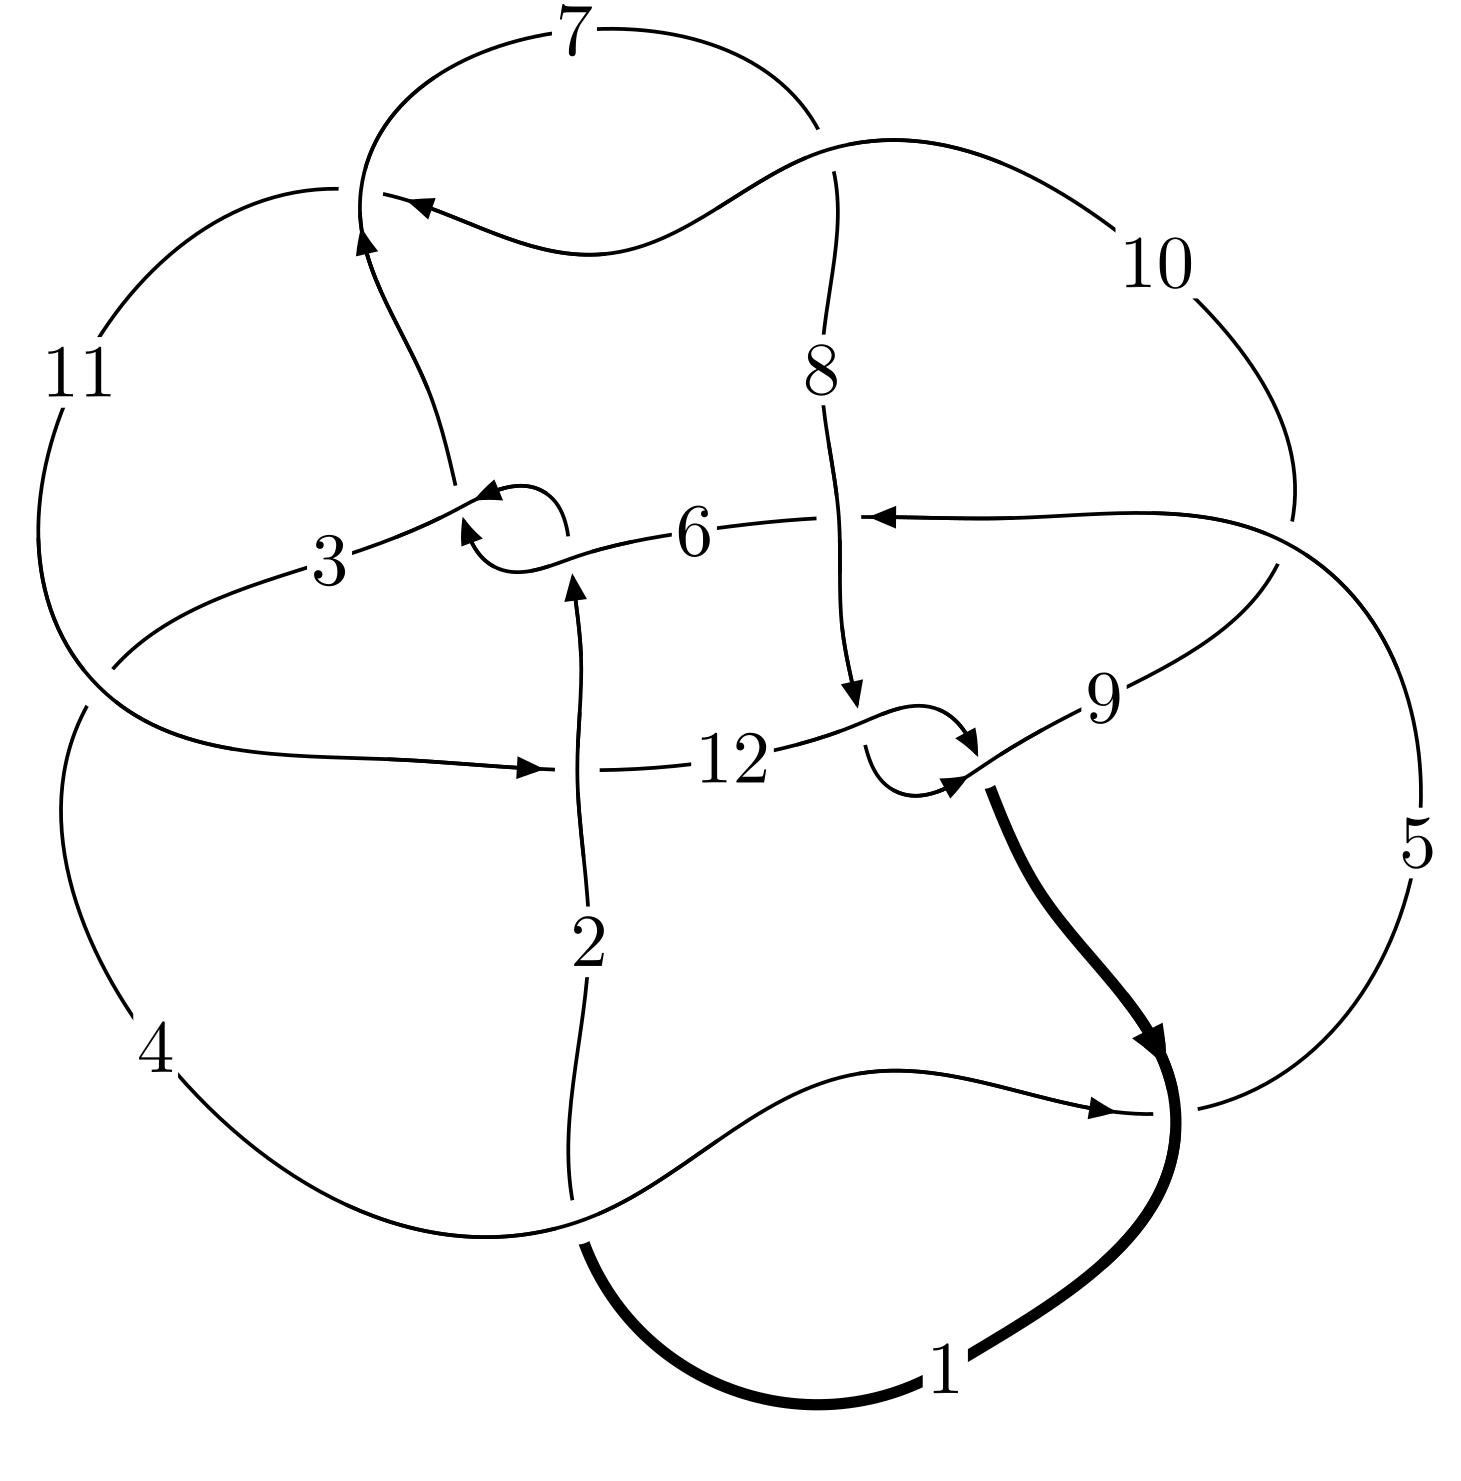
\includegraphics[width=112pt]{../../../GIT/diagram.site/Diagrams/png/1792_12a_0991.png}\\
\ \ \ A knot diagram\footnotemark}&
\allowdisplaybreaks
\textbf{Linearized knot diagam} \\
\cline{2-2}
 &
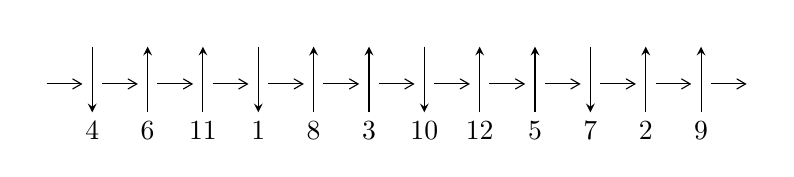
\begin{tikzpicture}[x=20pt, y=17pt]
	% nodes
	\node (C0) at (0, 0) {};
	\node (C1) at (1, 0) {};
	\node (C1U) at (1, +1) {};
	\node (C1D) at (1, -1) {4};

	\node (C2) at (2, 0) {};
	\node (C2U) at (2, +1) {};
	\node (C2D) at (2, -1) {6};

	\node (C3) at (3, 0) {};
	\node (C3U) at (3, +1) {};
	\node (C3D) at (3, -1) {11};

	\node (C4) at (4, 0) {};
	\node (C4U) at (4, +1) {};
	\node (C4D) at (4, -1) {1};

	\node (C5) at (5, 0) {};
	\node (C5U) at (5, +1) {};
	\node (C5D) at (5, -1) {8};

	\node (C6) at (6, 0) {};
	\node (C6U) at (6, +1) {};
	\node (C6D) at (6, -1) {3};

	\node (C7) at (7, 0) {};
	\node (C7U) at (7, +1) {};
	\node (C7D) at (7, -1) {10};

	\node (C8) at (8, 0) {};
	\node (C8U) at (8, +1) {};
	\node (C8D) at (8, -1) {12};

	\node (C9) at (9, 0) {};
	\node (C9U) at (9, +1) {};
	\node (C9D) at (9, -1) {5};

	\node (C10) at (10, 0) {};
	\node (C10U) at (10, +1) {};
	\node (C10D) at (10, -1) {7};

	\node (C11) at (11, 0) {};
	\node (C11U) at (11, +1) {};
	\node (C11D) at (11, -1) {2};

	\node (C12) at (12, 0) {};
	\node (C12U) at (12, +1) {};
	\node (C12D) at (12, -1) {9};
	\node (C13) at (13, 0) {};

	% arrows
	\draw[->,>={angle 60}]
	(C0) edge (C1) (C1) edge (C2) (C2) edge (C3) (C3) edge (C4) (C4) edge (C5) (C5) edge (C6) (C6) edge (C7) (C7) edge (C8) (C8) edge (C9) (C9) edge (C10) (C10) edge (C11) (C11) edge (C12) (C12) edge (C13) ;	\draw[->,>=stealth]
	(C1U) edge (C1D) (C2D) edge (C2U) (C3D) edge (C3U) (C4U) edge (C4D) (C5D) edge (C5U) (C6D) edge (C6U) (C7U) edge (C7D) (C8D) edge (C8U) (C9D) edge (C9U) (C10U) edge (C10D) (C11D) edge (C11U) (C12D) edge (C12U) ;
	\end{tikzpicture} \\
\hhline{~~} \\& 
\textbf{Solving Sequence} \\ \cline{2-2} 
 &
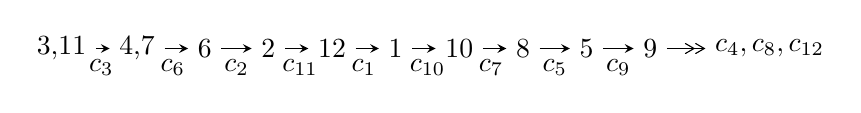
\begin{tikzpicture}[x=23pt, y=7pt]
	% node
	\node (A0) at (-1/8, 0) {3,11};
	\node (A1) at (17/16, 0) {4,7};
	\node (A2) at (17/8, 0) {6};
	\node (A3) at (25/8, 0) {2};
	\node (A4) at (33/8, 0) {12};
	\node (A5) at (41/8, 0) {1};
	\node (A6) at (49/8, 0) {10};
	\node (A7) at (57/8, 0) {8};
	\node (A8) at (65/8, 0) {5};
	\node (A9) at (73/8, 0) {9};
	\node (C1) at (1/2, -1) {$c_{3}$};
	\node (C2) at (13/8, -1) {$c_{6}$};
	\node (C3) at (21/8, -1) {$c_{2}$};
	\node (C4) at (29/8, -1) {$c_{11}$};
	\node (C5) at (37/8, -1) {$c_{1}$};
	\node (C6) at (45/8, -1) {$c_{10}$};
	\node (C7) at (53/8, -1) {$c_{7}$};
	\node (C8) at (61/8, -1) {$c_{5}$};
	\node (C9) at (69/8, -1) {$c_{9}$};
	\node (A10) at (11, 0) {$c_{4},c_{8},c_{12}$};

	% edge
	\draw[->,>=stealth]	
	(A0) edge (A1) (A1) edge (A2) (A2) edge (A3) (A3) edge (A4) (A4) edge (A5) (A5) edge (A6) (A6) edge (A7) (A7) edge (A8) (A8) edge (A9) ;
	\draw[->>,>={angle 60}]	
	(A9) edge (A10);
\end{tikzpicture} \\ 

\end{tabular} \\

\footnotetext{
The image of knot diagram is generated by the software ``\textbf{Draw programme}" developed by Andrew Bartholomew(\url{http://www.layer8.co.uk/maths/draw/index.htm\#Running-draw}), where we modified some parts for our purpose(\url{https://github.com/CATsTAILs/LinksPainter}).
}\phantom \\ \newline 
\centering \textbf{Ideals for irreducible components\footnotemark of $X_{\text{par}}$} 
 
\begin{align*}
I^u_{1}&=\langle 
57717367134771 u^{22}+147428293136959 u^{21}+\cdots+317082965674325 b+1212919831670806,\\
\phantom{I^u_{1}}&\phantom{= \langle  }-6.90652\times10^{14} u^{22}-9.73069\times10^{14} u^{21}+\cdots+6.02458\times10^{15} a-1.57925\times10^{16},\\
\phantom{I^u_{1}}&\phantom{= \langle  }u^{23}+3 u^{22}+\cdots+23 u+19\rangle \\
I^u_{2}&=\langle 
-1.43591\times10^{880} u^{123}+8.72577\times10^{878} u^{122}+\cdots+1.49298\times10^{884} b-1.12674\times10^{886},\\
\phantom{I^u_{2}}&\phantom{= \langle  }-1.05862\times10^{888} u^{123}+7.59549\times10^{887} u^{122}+\cdots+1.40244\times10^{891} a-1.54736\times10^{895},\\
\phantom{I^u_{2}}&\phantom{= \langle  }u^{124}-28 u^{122}+\cdots+37001253 u+9393563\rangle \\
I^u_{3}&=\langle 
u^4-2 u^3+2 u^2+b,\;u^4-2 u^3+u^2+a+2 u-1,\;u^5-3 u^4+4 u^3- u^2- u+1\rangle \\
I^u_{4}&=\langle 
3.38809\times10^{57} u^{37}+1.63783\times10^{58} u^{36}+\cdots+1.71599\times10^{58} b+1.67567\times10^{58},\\
\phantom{I^u_{4}}&\phantom{= \langle  }-6.22130\times10^{57} u^{37}-2.90017\times10^{58} u^{36}+\cdots+1.71599\times10^{58} a+2.01014\times10^{58},\;u^{38}+5 u^{37}+\cdots+3 u+1\rangle \\
\\
\end{align*}
\raggedright * 4 irreducible components of $\dim_{\mathbb{C}}=0$, with total 190 representations.\\
\footnotetext{All coefficients of polynomials are rational numbers. But the coefficients are sometimes approximated in decimal forms when there is not enough margin.}
\newpage
\renewcommand{\arraystretch}{1}
\centering \section*{I. $I^u_{1}= \langle 5.77\times10^{13} u^{22}+1.47\times10^{14} u^{21}+\cdots+3.17\times10^{14} b+1.21\times10^{15},\;-6.91\times10^{14} u^{22}-9.73\times10^{14} u^{21}+\cdots+6.02\times10^{15} a-1.58\times10^{16},\;u^{23}+3 u^{22}+\cdots+23 u+19 \rangle$}
\flushleft \textbf{(i) Arc colorings}\\
\begin{tabular}{m{7pt} m{180pt} m{7pt} m{180pt} }
\flushright $a_{3}=$&$\begin{pmatrix}1\\0\end{pmatrix}$ \\
\flushright $a_{11}=$&$\begin{pmatrix}0\\u\end{pmatrix}$ \\
\flushright $a_{4}=$&$\begin{pmatrix}1\\- u^2\end{pmatrix}$ \\
\flushright $a_{7}=$&$\begin{pmatrix}0.114639 u^{22}+0.161517 u^{21}+\cdots+0.233505 u+2.62135\\-0.182026 u^{22}-0.464952 u^{21}+\cdots-0.670669 u-3.82524\end{pmatrix}$ \\
\flushright $a_{6}=$&$\begin{pmatrix}0.296665 u^{22}+0.626468 u^{21}+\cdots+0.904173 u+6.44659\\-0.182026 u^{22}-0.464952 u^{21}+\cdots-0.670669 u-3.82524\end{pmatrix}$ \\
\flushright $a_{2}=$&$\begin{pmatrix}0.177816 u^{22}+0.437375 u^{21}+\cdots+1.33780 u+3.32029\\0.109266 u^{22}+0.0722014 u^{21}+\cdots+1.18417 u+0.352745\end{pmatrix}$ \\
\flushright $a_{12}=$&$\begin{pmatrix}0.297043 u^{22}+0.397846 u^{21}+\cdots+2.63301 u+2.54854\\-0.279180 u^{22}-0.505280 u^{21}+\cdots-2.85942 u-5.43579\end{pmatrix}$ \\
\flushright $a_{1}=$&$\begin{pmatrix}0.360217 u^{22}+0.803269 u^{21}+\cdots+1.35315 u+5.49844\\-0.115359 u^{22}-0.359386 u^{21}+\cdots+0.479691 u-3.09211\end{pmatrix}$ \\
\flushright $a_{10}=$&$\begin{pmatrix}-0.138170 u^{22}-0.231903 u^{21}+\cdots-2.84326 u-4.43308\\-0.351670 u^{22}-0.533545 u^{21}+\cdots-2.92986 u-5.45456\end{pmatrix}$ \\
\flushright $a_{8}=$&$\begin{pmatrix}-0.107726 u^{22}-0.111365 u^{21}+\cdots-0.581699 u-0.814060\\0.107088 u^{22}+0.280121 u^{21}+\cdots+2.38569 u+4.19317\end{pmatrix}$ \\
\flushright $a_{5}=$&$\begin{pmatrix}-0.0245807 u^{22}+0.151775 u^{21}+\cdots-5.03652 u+0.702173\\0.576947 u^{22}+1.14786 u^{21}+\cdots+3.46469 u+6.91005\end{pmatrix}$ \\
\flushright $a_{9}=$&$\begin{pmatrix}-0.363687 u^{22}-0.514114 u^{21}+\cdots-4.11079 u-4.90011\\0.231313 u^{22}+0.597069 u^{21}+\cdots+3.42987 u+5.50743\end{pmatrix}$\\&\end{tabular}
\flushleft \textbf{(ii) Obstruction class $= -1$}\\~\\
\flushleft \textbf{(iii) Cusp Shapes $= -\frac{81766888022974}{317082965674325} u^{22}-\frac{248859598527326}{317082965674325} u^{21}+\cdots+\frac{329686079723918}{317082965674325} u-\frac{784569176377574}{317082965674325}$}\\~\\
\newpage\renewcommand{\arraystretch}{1}
\flushleft \textbf{(iv) u-Polynomials at the component}\newline \\
\begin{tabular}{m{50pt}|m{274pt}}
Crossings & \hspace{64pt}u-Polynomials at each crossing \\
\hline $$\begin{aligned}c_{1},c_{4},c_{7}\\c_{10}\end{aligned}$$&$\begin{aligned}
&u^{23}- u^{22}+\cdots-7 u-1
\end{aligned}$\\
\hline $$\begin{aligned}c_{2},c_{6},c_{8}\\c_{12}\end{aligned}$$&$\begin{aligned}
&u^{23}- u^{22}+\cdots+12 u-4
\end{aligned}$\\
\hline $$\begin{aligned}c_{3},c_{9}\end{aligned}$$&$\begin{aligned}
&u^{23}-3 u^{22}+\cdots+23 u-19
\end{aligned}$\\
\hline $$\begin{aligned}c_{5},c_{11}\end{aligned}$$&$\begin{aligned}
&u^{23}+u^{22}+\cdots+31 u-1
\end{aligned}$\\
\hline
\end{tabular}\\~\\
\newpage\renewcommand{\arraystretch}{1}
\flushleft \textbf{(v) Riley Polynomials at the component}\newline \\
\begin{tabular}{m{50pt}|m{274pt}}
Crossings & \hspace{64pt}Riley Polynomials at each crossing \\
\hline $$\begin{aligned}c_{1},c_{4},c_{7}\\c_{10}\end{aligned}$$&$\begin{aligned}
&y^{23}+27 y^{22}+\cdots+25 y-1
\end{aligned}$\\
\hline $$\begin{aligned}c_{2},c_{6},c_{8}\\c_{12}\end{aligned}$$&$\begin{aligned}
&y^{23}-15 y^{22}+\cdots+96 y-16
\end{aligned}$\\
\hline $$\begin{aligned}c_{3},c_{9}\end{aligned}$$&$\begin{aligned}
&y^{23}-17 y^{22}+\cdots+301 y-361
\end{aligned}$\\
\hline $$\begin{aligned}c_{5},c_{11}\end{aligned}$$&$\begin{aligned}
&y^{23}+11 y^{22}+\cdots+957 y-1
\end{aligned}$\\
\hline
\end{tabular}\\~\\
\newpage\flushleft \textbf{(vi) Complex Volumes and Cusp Shapes}
$$\begin{array}{c|c|c}  
\text{Solutions to }I^u_{1}& \I (\text{vol} + \sqrt{-1}CS) & \text{Cusp shape}\\
 \hline 
\begin{aligned}
u &= \phantom{-}0.918917 + 0.525926 I \\
a &= -0.588465 + 0.739338 I \\
b &= \phantom{-}1.177530 + 0.446851 I\end{aligned}
 & \phantom{-}2.51017 + 8.14058 I & \phantom{-}6.64567 - 9.11727 I \\ \hline\begin{aligned}
u &= \phantom{-}0.918917 - 0.525926 I \\
a &= -0.588465 - 0.739338 I \\
b &= \phantom{-}1.177530 - 0.446851 I\end{aligned}
 & \phantom{-}2.51017 - 8.14058 I & \phantom{-}6.64567 + 9.11727 I \\ \hline\begin{aligned}
u &= \phantom{-}0.773342 + 0.494667 I \\
a &= -1.04701 - 1.59683 I \\
b &= -0.957225 - 0.497796 I\end{aligned}
 & \phantom{-}9.76931 + 4.11749 I & \phantom{-}5.17924 - 6.62141 I \\ \hline\begin{aligned}
u &= \phantom{-}0.773342 - 0.494667 I \\
a &= -1.04701 + 1.59683 I \\
b &= -0.957225 + 0.497796 I\end{aligned}
 & \phantom{-}9.76931 - 4.11749 I & \phantom{-}5.17924 + 6.62141 I \\ \hline\begin{aligned}
u &= -0.871157\phantom{ +0.000000I} \\
a &= \phantom{-}0.623723\phantom{ +0.000000I} \\
b &= -0.717781\phantom{ +0.000000I}\end{aligned}
 & \phantom{-}1.42427\phantom{ +0.000000I} & \phantom{-}5.58020\phantom{ +0.000000I} \\ \hline\begin{aligned}
u &= \phantom{-}1.054960 + 0.459775 I \\
a &= \phantom{-}0.215920 - 0.029509 I \\
b &= -1.042380 + 0.452100 I\end{aligned}
 & \phantom{-}2.25624 - 3.72277 I & \phantom{-}3.77679 + 4.53205 I \\ \hline\begin{aligned}
u &= \phantom{-}1.054960 - 0.459775 I \\
a &= \phantom{-}0.215920 + 0.029509 I \\
b &= -1.042380 - 0.452100 I\end{aligned}
 & \phantom{-}2.25624 + 3.72277 I & \phantom{-}3.77679 - 4.53205 I \\ \hline\begin{aligned}
u &= -1.197360 + 0.107009 I \\
a &= \phantom{-}0.186498 - 1.278020 I \\
b &= \phantom{-}1.223500 - 0.651345 I\end{aligned}
 & \phantom{-}13.7533 - 3.8768 I & \phantom{-}14.9082 + 3.5373 I \\ \hline\begin{aligned}
u &= -1.197360 - 0.107009 I \\
a &= \phantom{-}0.186498 + 1.278020 I \\
b &= \phantom{-}1.223500 + 0.651345 I\end{aligned}
 & \phantom{-}13.7533 + 3.8768 I & \phantom{-}14.9082 - 3.5373 I \\ \hline\begin{aligned}
u &= \phantom{-}0.271747 + 0.746918 I \\
a &= \phantom{-}0.385059 - 0.712732 I \\
b &= \phantom{-}0.402904 - 0.603471 I\end{aligned}
 & -2.39867 - 0.27896 I & -3.60170 + 1.81372 I\\
 \hline 
 \end{array}$$\newpage$$\begin{array}{c|c|c}  
\text{Solutions to }I^u_{1}& \I (\text{vol} + \sqrt{-1}CS) & \text{Cusp shape}\\
 \hline 
\begin{aligned}
u &= \phantom{-}0.271747 - 0.746918 I \\
a &= \phantom{-}0.385059 + 0.712732 I \\
b &= \phantom{-}0.402904 + 0.603471 I\end{aligned}
 & -2.39867 + 0.27896 I & -3.60170 - 1.81372 I \\ \hline\begin{aligned}
u &= -1.189060 + 0.477242 I \\
a &= \phantom{-}0.268653 - 1.237180 I \\
b &= \phantom{-}1.152630 - 0.048406 I\end{aligned}
 & \phantom{-}12.93090 - 1.19686 I & \phantom{-}14.2711 + 0.3658 I \\ \hline\begin{aligned}
u &= -1.189060 - 0.477242 I \\
a &= \phantom{-}0.268653 + 1.237180 I \\
b &= \phantom{-}1.152630 + 0.048406 I\end{aligned}
 & \phantom{-}12.93090 + 1.19686 I & \phantom{-}14.2711 - 0.3658 I \\ \hline\begin{aligned}
u &= -1.203270 + 0.495710 I \\
a &= \phantom{-}0.175292 - 1.080310 I \\
b &= -0.066343 - 1.107590 I\end{aligned}
 & \phantom{-}6.02936 - 6.98335 I & \phantom{-}8.21274 + 5.05079 I \\ \hline\begin{aligned}
u &= -1.203270 - 0.495710 I \\
a &= \phantom{-}0.175292 + 1.080310 I \\
b &= -0.066343 + 1.107590 I\end{aligned}
 & \phantom{-}6.02936 + 6.98335 I & \phantom{-}8.21274 - 5.05079 I \\ \hline\begin{aligned}
u &= -0.211749 + 0.550582 I \\
a &= \phantom{-}1.008340 - 0.441111 I \\
b &= -0.357064 + 0.362726 I\end{aligned}
 & \phantom{-}1.04800 - 1.12978 I & \phantom{-}8.64416 + 6.06289 I \\ \hline\begin{aligned}
u &= -0.211749 - 0.550582 I \\
a &= \phantom{-}1.008340 + 0.441111 I \\
b &= -0.357064 - 0.362726 I\end{aligned}
 & \phantom{-}1.04800 + 1.12978 I & \phantom{-}8.64416 - 6.06289 I \\ \hline\begin{aligned}
u &= -0.41447 + 1.35905 I \\
a &= -0.698894 + 0.209343 I \\
b &= -1.220420 - 0.208268 I\end{aligned}
 & \phantom{-}6.27657 + 2.79434 I & \phantom{-}13.30273 - 3.14397 I \\ \hline\begin{aligned}
u &= -0.41447 - 1.35905 I \\
a &= -0.698894 - 0.209343 I \\
b &= -1.220420 + 0.208268 I\end{aligned}
 & \phantom{-}6.27657 - 2.79434 I & \phantom{-}13.30273 + 3.14397 I \\ \hline\begin{aligned}
u &= \phantom{-}1.73548 + 0.04257 I \\
a &= -0.126978 - 0.685204 I \\
b &= \phantom{-}0.971727 - 0.746612 I\end{aligned}
 & \phantom{-}6.49002 - 5.81139 I & \phantom{-}9.27142 + 6.06710 I\\
 \hline 
 \end{array}$$\newpage$$\begin{array}{c|c|c}  
\text{Solutions to }I^u_{1}& \I (\text{vol} + \sqrt{-1}CS) & \text{Cusp shape}\\
 \hline 
\begin{aligned}
u &= \phantom{-}1.73548 - 0.04257 I \\
a &= -0.126978 + 0.685204 I \\
b &= \phantom{-}0.971727 + 0.746612 I\end{aligned}
 & \phantom{-}6.49002 + 5.81139 I & \phantom{-}9.27142 - 6.06710 I \\ \hline\begin{aligned}
u &= -1.60297 + 0.82134 I \\
a &= -0.142907 + 0.899405 I \\
b &= -1.42596 + 0.57620 I\end{aligned}
 & \phantom{-}14.6447 - 19.3062 I & \phantom{-}11.5995 + 8.9972 I \\ \hline\begin{aligned}
u &= -1.60297 - 0.82134 I \\
a &= -0.142907 - 0.899405 I \\
b &= -1.42596 - 0.57620 I\end{aligned}
 & \phantom{-}14.6447 + 19.3062 I & \phantom{-}11.5995 - 8.9972 I\\
 \hline 
 \end{array}$$\newpage\newpage\renewcommand{\arraystretch}{1}
\centering \section*{II. $I^u_{2}= \langle -1.44\times10^{880} u^{123}+8.73\times10^{878} u^{122}+\cdots+1.49\times10^{884} b-1.13\times10^{886},\;-1.06\times10^{888} u^{123}+7.60\times10^{887} u^{122}+\cdots+1.40\times10^{891} a-1.55\times10^{895},\;u^{124}-28 u^{122}+\cdots+37001253 u+9393563 \rangle$}
\flushleft \textbf{(i) Arc colorings}\\
\begin{tabular}{m{7pt} m{180pt} m{7pt} m{180pt} }
\flushright $a_{3}=$&$\begin{pmatrix}1\\0\end{pmatrix}$ \\
\flushright $a_{11}=$&$\begin{pmatrix}0\\u\end{pmatrix}$ \\
\flushright $a_{4}=$&$\begin{pmatrix}1\\- u^2\end{pmatrix}$ \\
\flushright $a_{7}=$&$\begin{pmatrix}0.000754843 u^{123}-0.000541592 u^{122}+\cdots+27659.3 u+11033.4\\0.0000961780 u^{123}-5.84455\times10^{-6} u^{122}+\cdots-1187.04 u+75.4696\end{pmatrix}$ \\
\flushright $a_{6}=$&$\begin{pmatrix}0.000658665 u^{123}-0.000535748 u^{122}+\cdots+28846.3 u+10957.9\\0.0000961780 u^{123}-5.84455\times10^{-6} u^{122}+\cdots-1187.04 u+75.4696\end{pmatrix}$ \\
\flushright $a_{2}=$&$\begin{pmatrix}-0.000769260 u^{123}+0.000478016 u^{122}+\cdots-24948.3 u-10481.1\\-0.0000934100 u^{123}+0.0000559721 u^{122}+\cdots-1937.68 u-853.277\end{pmatrix}$ \\
\flushright $a_{12}=$&$\begin{pmatrix}-0.00286019 u^{123}+0.00209707 u^{122}+\cdots-102095. u-39638.9\\0.000606344 u^{123}-0.000421349 u^{122}+\cdots+22961.5 u+9239.15\end{pmatrix}$ \\
\flushright $a_{1}=$&$\begin{pmatrix}-0.00119794 u^{123}+0.000731324 u^{122}+\cdots-37347.0 u-15824.6\\0.0000980954 u^{123}-0.0000512982 u^{122}+\cdots+3408.16 u+1526.19\end{pmatrix}$ \\
\flushright $a_{10}=$&$\begin{pmatrix}-0.00205809 u^{123}+0.00151971 u^{122}+\cdots-72999.2 u-28236.8\\0.000533988 u^{123}-0.000385230 u^{122}+\cdots+20585.5 u+8103.55\end{pmatrix}$ \\
\flushright $a_{8}=$&$\begin{pmatrix}0.00179696 u^{123}-0.00153781 u^{122}+\cdots+64535.5 u+22832.9\\-0.00121549 u^{123}+0.000954177 u^{122}+\cdots-46498.2 u-17482.4\end{pmatrix}$ \\
\flushright $a_{5}=$&$\begin{pmatrix}0.00114349 u^{123}-0.000867960 u^{122}+\cdots+37250.0 u+14109.5\\-0.000621780 u^{123}+0.000410335 u^{122}+\cdots-18252.1 u-7479.59\end{pmatrix}$ \\
\flushright $a_{9}=$&$\begin{pmatrix}-0.00197358 u^{123}+0.00136446 u^{122}+\cdots-71871.7 u-28676.8\\0.000155176 u^{123}-0.0000592743 u^{122}+\cdots+5180.54 u+2527.54\end{pmatrix}$\\&\end{tabular}
\flushleft \textbf{(ii) Obstruction class $= -1$}\\~\\
\flushleft \textbf{(iii) Cusp Shapes $= -0.00308181 u^{123}+0.00229861 u^{122}+\cdots-103573. u-40396.6$}\\~\\
\newpage\renewcommand{\arraystretch}{1}
\flushleft \textbf{(iv) u-Polynomials at the component}\newline \\
\begin{tabular}{m{50pt}|m{274pt}}
Crossings & \hspace{64pt}u-Polynomials at each crossing \\
\hline $$\begin{aligned}c_{1},c_{4},c_{7}\\c_{10}\end{aligned}$$&$\begin{aligned}
&u^{124}-8 u^{123}+\cdots-19679 u-1829
\end{aligned}$\\
\hline $$\begin{aligned}c_{2},c_{6},c_{8}\\c_{12}\end{aligned}$$&$\begin{aligned}
&u^{124}-3 u^{123}+\cdots+13060 u-7061
\end{aligned}$\\
\hline $$\begin{aligned}c_{3},c_{9}\end{aligned}$$&$\begin{aligned}
&u^{124}-28 u^{122}+\cdots-37001253 u+9393563
\end{aligned}$\\
\hline $$\begin{aligned}c_{5},c_{11}\end{aligned}$$&$\begin{aligned}
&u^{124}+12 u^{123}+\cdots-23079 u+2117
\end{aligned}$\\
\hline
\end{tabular}\\~\\
\newpage\renewcommand{\arraystretch}{1}
\flushleft \textbf{(v) Riley Polynomials at the component}\newline \\
\begin{tabular}{m{50pt}|m{274pt}}
Crossings & \hspace{64pt}Riley Polynomials at each crossing \\
\hline $$\begin{aligned}c_{1},c_{4},c_{7}\\c_{10}\end{aligned}$$&$\begin{aligned}
&y^{124}+104 y^{123}+\cdots-374690495 y+3345241
\end{aligned}$\\
\hline $$\begin{aligned}c_{2},c_{6},c_{8}\\c_{12}\end{aligned}$$&$\begin{aligned}
&y^{124}-85 y^{123}+\cdots-834961334 y+49857721
\end{aligned}$\\
\hline $$\begin{aligned}c_{3},c_{9}\end{aligned}$$&$\begin{aligned}
&y^{124}-56 y^{123}+\cdots-7183023354678805 y+88239025834969
\end{aligned}$\\
\hline $$\begin{aligned}c_{5},c_{11}\end{aligned}$$&$\begin{aligned}
&y^{124}-36 y^{123}+\cdots+1058022751 y+4481689
\end{aligned}$\\
\hline
\end{tabular}\\~\\
\newpage\flushleft \textbf{(vi) Complex Volumes and Cusp Shapes}
$$\begin{array}{c|c|c}  
\text{Solutions to }I^u_{2}& \I (\text{vol} + \sqrt{-1}CS) & \text{Cusp shape}\\
 \hline 
\begin{aligned}
u &= -0.832257 + 0.559566 I \\
a &= -0.78785 + 1.31337 I \\
b &= -1.50165 + 0.80491 I\end{aligned}
 & \phantom{-}11.54920 - 3.29623 I & \phantom{-0.000000 } 0 \\ \hline\begin{aligned}
u &= -0.832257 - 0.559566 I \\
a &= -0.78785 - 1.31337 I \\
b &= -1.50165 - 0.80491 I\end{aligned}
 & \phantom{-}11.54920 + 3.29623 I & \phantom{-0.000000 } 0 \\ \hline\begin{aligned}
u &= -0.991089 + 0.153659 I \\
a &= -0.169531 + 1.156440 I \\
b &= -0.151031 + 1.398850 I\end{aligned}
 & \phantom{-}2.48023 - 1.03604 I & \phantom{-0.000000 } 0 \\ \hline\begin{aligned}
u &= -0.991089 - 0.153659 I \\
a &= -0.169531 - 1.156440 I \\
b &= -0.151031 - 1.398850 I\end{aligned}
 & \phantom{-}2.48023 + 1.03604 I & \phantom{-0.000000 } 0 \\ \hline\begin{aligned}
u &= \phantom{-}0.898023 + 0.383481 I \\
a &= \phantom{-}0.934050 + 0.338258 I \\
b &= -0.975376 + 0.111434 I\end{aligned}
 & \phantom{-}1.73213 - 0.66883 I & \phantom{-0.000000 } 0 \\ \hline\begin{aligned}
u &= \phantom{-}0.898023 - 0.383481 I \\
a &= \phantom{-}0.934050 - 0.338258 I \\
b &= -0.975376 - 0.111434 I\end{aligned}
 & \phantom{-}1.73213 + 0.66883 I & \phantom{-0.000000 } 0 \\ \hline\begin{aligned}
u &= -0.929923 + 0.254749 I \\
a &= \phantom{-}0.17250 + 1.73396 I \\
b &= -1.46751 + 0.15284 I\end{aligned}
 & \phantom{-}14.7335 - 8.0221 I & \phantom{-0.000000 } 0 \\ \hline\begin{aligned}
u &= -0.929923 - 0.254749 I \\
a &= \phantom{-}0.17250 - 1.73396 I \\
b &= -1.46751 - 0.15284 I\end{aligned}
 & \phantom{-}14.7335 + 8.0221 I & \phantom{-0.000000 } 0 \\ \hline\begin{aligned}
u &= -1.031240 + 0.210849 I \\
a &= \phantom{-}0.271925 - 1.250820 I \\
b &= \phantom{-}1.58994 - 0.52839 I\end{aligned}
 & \phantom{-}15.1848 + 6.0579 I & \phantom{-0.000000 } 0 \\ \hline\begin{aligned}
u &= -1.031240 - 0.210849 I \\
a &= \phantom{-}0.271925 + 1.250820 I \\
b &= \phantom{-}1.58994 + 0.52839 I\end{aligned}
 & \phantom{-}15.1848 - 6.0579 I & \phantom{-0.000000 } 0\\
 \hline 
 \end{array}$$\newpage$$\begin{array}{c|c|c}  
\text{Solutions to }I^u_{2}& \I (\text{vol} + \sqrt{-1}CS) & \text{Cusp shape}\\
 \hline 
\begin{aligned}
u &= \phantom{-}0.897036 + 0.586814 I \\
a &= -0.91039 - 1.09007 I \\
b &= -0.453265 - 0.603763 I\end{aligned}
 & \phantom{-}9.66429 + 4.09208 I & \phantom{-0.000000 } 0 \\ \hline\begin{aligned}
u &= \phantom{-}0.897036 - 0.586814 I \\
a &= -0.91039 + 1.09007 I \\
b &= -0.453265 + 0.603763 I\end{aligned}
 & \phantom{-}9.66429 - 4.09208 I & \phantom{-0.000000 } 0 \\ \hline\begin{aligned}
u &= -0.920705 + 0.549630 I \\
a &= \phantom{-}1.068840 + 0.794345 I \\
b &= -1.226030 + 0.134089 I\end{aligned}
 & \phantom{-}9.85131 + 0.58116 I & \phantom{-0.000000 } 0 \\ \hline\begin{aligned}
u &= -0.920705 - 0.549630 I \\
a &= \phantom{-}1.068840 - 0.794345 I \\
b &= -1.226030 - 0.134089 I\end{aligned}
 & \phantom{-}9.85131 - 0.58116 I & \phantom{-0.000000 } 0 \\ \hline\begin{aligned}
u &= -1.060230 + 0.182661 I \\
a &= -1.034840 + 0.100779 I \\
b &= \phantom{-}1.286310 - 0.336100 I\end{aligned}
 & \phantom{-}6.30482 - 3.83713 I & \phantom{-0.000000 } 0 \\ \hline\begin{aligned}
u &= -1.060230 - 0.182661 I \\
a &= -1.034840 - 0.100779 I \\
b &= \phantom{-}1.286310 + 0.336100 I\end{aligned}
 & \phantom{-}6.30482 + 3.83713 I & \phantom{-0.000000 } 0 \\ \hline\begin{aligned}
u &= \phantom{-}0.828661 + 0.396010 I \\
a &= -0.55923 - 1.82969 I \\
b &= -1.245570 - 0.396965 I\end{aligned}
 & \phantom{-}9.66429 + 4.09208 I & \phantom{-0.000000 } 0 \\ \hline\begin{aligned}
u &= \phantom{-}0.828661 - 0.396010 I \\
a &= -0.55923 + 1.82969 I \\
b &= -1.245570 + 0.396965 I\end{aligned}
 & \phantom{-}9.66429 - 4.09208 I & \phantom{-0.000000 } 0 \\ \hline\begin{aligned}
u &= \phantom{-}0.591720 + 0.675350 I \\
a &= \phantom{-}0.941129 - 0.041225 I \\
b &= \phantom{-}0.027565 - 0.660549 I\end{aligned}
 & \phantom{-}2.35447 + 0.13282 I & \phantom{-0.000000 } 0 \\ \hline\begin{aligned}
u &= \phantom{-}0.591720 - 0.675350 I \\
a &= \phantom{-}0.941129 + 0.041225 I \\
b &= \phantom{-}0.027565 + 0.660549 I\end{aligned}
 & \phantom{-}2.35447 - 0.13282 I & \phantom{-0.000000 } 0\\
 \hline 
 \end{array}$$\newpage$$\begin{array}{c|c|c}  
\text{Solutions to }I^u_{2}& \I (\text{vol} + \sqrt{-1}CS) & \text{Cusp shape}\\
 \hline 
\begin{aligned}
u &= -0.761610 + 0.474972 I \\
a &= -0.779793 - 0.961860 I \\
b &= \phantom{-}1.035030 - 0.335104 I\end{aligned}
 & -0.49565 - 3.43639 I & \phantom{-0.000000 } 0 \\ \hline\begin{aligned}
u &= -0.761610 - 0.474972 I \\
a &= -0.779793 + 0.961860 I \\
b &= \phantom{-}1.035030 + 0.335104 I\end{aligned}
 & -0.49565 + 3.43639 I & \phantom{-0.000000 } 0 \\ \hline\begin{aligned}
u &= -0.853877 + 0.242911 I \\
a &= -0.20805 + 1.49543 I \\
b &= \phantom{-}0.045866 + 1.387410 I\end{aligned}
 & \phantom{-}3.86911 - 6.05067 I & \phantom{-0.000000 } 0 \\ \hline\begin{aligned}
u &= -0.853877 - 0.242911 I \\
a &= -0.20805 - 1.49543 I \\
b &= \phantom{-}0.045866 - 1.387410 I\end{aligned}
 & \phantom{-}3.86911 + 6.05067 I & \phantom{-0.000000 } 0 \\ \hline\begin{aligned}
u &= -0.378616 + 0.799354 I \\
a &= \phantom{-}1.026480 - 0.036530 I \\
b &= \phantom{-}0.323754 + 0.441607 I\end{aligned}
 & \phantom{-}1.73213 - 0.66883 I & \phantom{-0.000000 } 0 \\ \hline\begin{aligned}
u &= -0.378616 - 0.799354 I \\
a &= \phantom{-}1.026480 + 0.036530 I \\
b &= \phantom{-}0.323754 - 0.441607 I\end{aligned}
 & \phantom{-}1.73213 + 0.66883 I & \phantom{-0.000000 } 0 \\ \hline\begin{aligned}
u &= -0.873073 + 0.016053 I \\
a &= \phantom{-}0.623181 + 0.019412 I \\
b &= -0.719342 + 0.035275 I\end{aligned}
 & \phantom{-}1.42426\phantom{ +0.000000I} & \phantom{-0.000000 } 0 \\ \hline\begin{aligned}
u &= -0.873073 - 0.016053 I \\
a &= \phantom{-}0.623181 - 0.019412 I \\
b &= -0.719342 - 0.035275 I\end{aligned}
 & \phantom{-}1.42426\phantom{ +0.000000I} & \phantom{-0.000000 } 0 \\ \hline\begin{aligned}
u &= \phantom{-}1.100840 + 0.251619 I \\
a &= \phantom{-}0.239334 + 1.247970 I \\
b &= \phantom{-}1.40521 + 0.43298 I\end{aligned}
 & \phantom{-}10.89050 - 1.43238 I & \phantom{-0.000000 } 0 \\ \hline\begin{aligned}
u &= \phantom{-}1.100840 - 0.251619 I \\
a &= \phantom{-}0.239334 - 1.247970 I \\
b &= \phantom{-}1.40521 - 0.43298 I\end{aligned}
 & \phantom{-}10.89050 + 1.43238 I & \phantom{-0.000000 } 0\\
 \hline 
 \end{array}$$\newpage$$\begin{array}{c|c|c}  
\text{Solutions to }I^u_{2}& \I (\text{vol} + \sqrt{-1}CS) & \text{Cusp shape}\\
 \hline 
\begin{aligned}
u &= \phantom{-}0.863941 + 0.098745 I \\
a &= -0.065027 - 1.127290 I \\
b &= -0.526831 - 1.287540 I\end{aligned}
 & \phantom{-}2.80036 + 3.42863 I & \phantom{-0.000000 } 0 \\ \hline\begin{aligned}
u &= \phantom{-}0.863941 - 0.098745 I \\
a &= -0.065027 + 1.127290 I \\
b &= -0.526831 + 1.287540 I\end{aligned}
 & \phantom{-}2.80036 - 3.42863 I & \phantom{-0.000000 } 0 \\ \hline\begin{aligned}
u &= \phantom{-}0.842414 + 0.194962 I \\
a &= -0.04701 - 1.43734 I \\
b &= \phantom{-}0.047595 - 1.090590 I\end{aligned}
 & \phantom{-}1.03606 + 2.94499 I & \phantom{-0.000000 } 0 \\ \hline\begin{aligned}
u &= \phantom{-}0.842414 - 0.194962 I \\
a &= -0.04701 + 1.43734 I \\
b &= \phantom{-}0.047595 + 1.090590 I\end{aligned}
 & \phantom{-}1.03606 - 2.94499 I & \phantom{-0.000000 } 0 \\ \hline\begin{aligned}
u &= -1.100520 + 0.307549 I \\
a &= \phantom{-}0.583930 - 0.874030 I \\
b &= -0.583330 - 0.133203 I\end{aligned}
 & \phantom{-}4.49764 + 3.55654 I & \phantom{-0.000000 } 0 \\ \hline\begin{aligned}
u &= -1.100520 - 0.307549 I \\
a &= \phantom{-}0.583930 + 0.874030 I \\
b &= -0.583330 + 0.133203 I\end{aligned}
 & \phantom{-}4.49764 - 3.55654 I & \phantom{-0.000000 } 0 \\ \hline\begin{aligned}
u &= \phantom{-}1.159350 + 0.196439 I \\
a &= -0.678596 - 0.156815 I \\
b &= \phantom{-}1.169790 + 0.264504 I\end{aligned}
 & \phantom{-}4.49764 + 3.55654 I & \phantom{-0.000000 } 0 \\ \hline\begin{aligned}
u &= \phantom{-}1.159350 - 0.196439 I \\
a &= -0.678596 + 0.156815 I \\
b &= \phantom{-}1.169790 - 0.264504 I\end{aligned}
 & \phantom{-}4.49764 - 3.55654 I & \phantom{-0.000000 } 0 \\ \hline\begin{aligned}
u &= \phantom{-}0.827945 + 0.838917 I \\
a &= -0.328047 + 0.701006 I \\
b &= \phantom{-}0.321299 + 0.492971 I\end{aligned}
 & \phantom{-}5.37387 - 2.54528 I & \phantom{-0.000000 } 0 \\ \hline\begin{aligned}
u &= \phantom{-}0.827945 - 0.838917 I \\
a &= -0.328047 - 0.701006 I \\
b &= \phantom{-}0.321299 - 0.492971 I\end{aligned}
 & \phantom{-}5.37387 + 2.54528 I & \phantom{-0.000000 } 0\\
 \hline 
 \end{array}$$\newpage$$\begin{array}{c|c|c}  
\text{Solutions to }I^u_{2}& \I (\text{vol} + \sqrt{-1}CS) & \text{Cusp shape}\\
 \hline 
\begin{aligned}
u &= -0.426039 + 0.695884 I \\
a &= \phantom{-}0.265031 + 0.619278 I \\
b &= \phantom{-}0.208538 + 0.852829 I\end{aligned}
 & -0.49565 - 3.43639 I & \phantom{-0.000000 } 0 \\ \hline\begin{aligned}
u &= -0.426039 - 0.695884 I \\
a &= \phantom{-}0.265031 - 0.619278 I \\
b &= \phantom{-}0.208538 - 0.852829 I\end{aligned}
 & -0.49565 + 3.43639 I & \phantom{-0.000000 } 0 \\ \hline\begin{aligned}
u &= \phantom{-}0.673227 + 0.448450 I \\
a &= \phantom{-}0.30754 + 1.72391 I \\
b &= \phantom{-}1.142750 - 0.092130 I\end{aligned}
 & \phantom{-}4.72714 - 2.47544 I & \phantom{-0.000000 } 0 \\ \hline\begin{aligned}
u &= \phantom{-}0.673227 - 0.448450 I \\
a &= \phantom{-}0.30754 - 1.72391 I \\
b &= \phantom{-}1.142750 + 0.092130 I\end{aligned}
 & \phantom{-}4.72714 + 2.47544 I & \phantom{-0.000000 } 0 \\ \hline\begin{aligned}
u &= -0.777970 + 0.911853 I \\
a &= -0.333951 - 0.593460 I \\
b &= -0.185475 - 0.437289 I\end{aligned}
 & \phantom{-}1.03606 - 2.94499 I & \phantom{-0.000000 } 0 \\ \hline\begin{aligned}
u &= -0.777970 - 0.911853 I \\
a &= -0.333951 + 0.593460 I \\
b &= -0.185475 + 0.437289 I\end{aligned}
 & \phantom{-}1.03606 + 2.94499 I & \phantom{-0.000000 } 0 \\ \hline\begin{aligned}
u &= \phantom{-}0.777489\phantom{ +0.000000I} \\
a &= -1.74454\phantom{ +0.000000I} \\
b &= \phantom{-}1.17395\phantom{ +0.000000I}\end{aligned}
 & \phantom{-}5.52857\phantom{ +0.000000I} & \phantom{-0.000000 } 0 \\ \hline\begin{aligned}
u &= \phantom{-}0.832394 + 0.895367 I \\
a &= -0.387083 + 0.564279 I \\
b &= -0.173857 + 0.721043 I\end{aligned}
 & \phantom{-}5.27011 + 8.68957 I & \phantom{-0.000000 } 0 \\ \hline\begin{aligned}
u &= \phantom{-}0.832394 - 0.895367 I \\
a &= -0.387083 - 0.564279 I \\
b &= -0.173857 - 0.721043 I\end{aligned}
 & \phantom{-}5.27011 - 8.68957 I & \phantom{-0.000000 } 0 \\ \hline\begin{aligned}
u &= \phantom{-}1.157570 + 0.478481 I \\
a &= \phantom{-}0.169523 + 1.120890 I \\
b &= \phantom{-}0.004007 + 1.271680 I\end{aligned}
 & \phantom{-}10.0846 + 12.8687 I & \phantom{-0.000000 } 0\\
 \hline 
 \end{array}$$\newpage$$\begin{array}{c|c|c}  
\text{Solutions to }I^u_{2}& \I (\text{vol} + \sqrt{-1}CS) & \text{Cusp shape}\\
 \hline 
\begin{aligned}
u &= \phantom{-}1.157570 - 0.478481 I \\
a &= \phantom{-}0.169523 - 1.120890 I \\
b &= \phantom{-}0.004007 - 1.271680 I\end{aligned}
 & \phantom{-}10.0846 - 12.8687 I & \phantom{-0.000000 } 0 \\ \hline\begin{aligned}
u &= -1.239930 + 0.197630 I \\
a &= \phantom{-}0.099971 + 0.900563 I \\
b &= -0.842102 + 0.645976 I\end{aligned}
 & \phantom{-}4.38491 - 3.32315 I & \phantom{-0.000000 } 0 \\ \hline\begin{aligned}
u &= -1.239930 - 0.197630 I \\
a &= \phantom{-}0.099971 - 0.900563 I \\
b &= -0.842102 - 0.645976 I\end{aligned}
 & \phantom{-}4.38491 + 3.32315 I & \phantom{-0.000000 } 0 \\ \hline\begin{aligned}
u &= -0.657674 + 1.073390 I \\
a &= \phantom{-}0.752991 - 0.858738 I \\
b &= \phantom{-}1.072340 - 0.138901 I\end{aligned}
 & \phantom{-}2.74503 - 3.72225 I & \phantom{-0.000000 } 0 \\ \hline\begin{aligned}
u &= -0.657674 - 1.073390 I \\
a &= \phantom{-}0.752991 + 0.858738 I \\
b &= \phantom{-}1.072340 + 0.138901 I\end{aligned}
 & \phantom{-}2.74503 + 3.72225 I & \phantom{-0.000000 } 0 \\ \hline\begin{aligned}
u &= \phantom{-}0.733914\phantom{ +0.000000I} \\
a &= \phantom{-}0.120487\phantom{ +0.000000I} \\
b &= -1.40350\phantom{ +0.000000I}\end{aligned}
 & \phantom{-}5.52857\phantom{ +0.000000I} & \phantom{-0.000000 } 0 \\ \hline\begin{aligned}
u &= \phantom{-}1.182510 + 0.452565 I \\
a &= -0.190383 - 1.066910 I \\
b &= -1.48441 - 0.65466 I\end{aligned}
 & \phantom{-}6.84626 + 6.36165 I & \phantom{-0.000000 } 0 \\ \hline\begin{aligned}
u &= \phantom{-}1.182510 - 0.452565 I \\
a &= -0.190383 + 1.066910 I \\
b &= -1.48441 + 0.65466 I\end{aligned}
 & \phantom{-}6.84626 - 6.36165 I & \phantom{-0.000000 } 0 \\ \hline\begin{aligned}
u &= \phantom{-}0.447520 + 1.187290 I \\
a &= -0.956824 + 0.107479 I \\
b &= \phantom{-}0.508576 + 0.294345 I\end{aligned}
 & \phantom{-}7.69733 - 7.68655 I & \phantom{-0.000000 } 0 \\ \hline\begin{aligned}
u &= \phantom{-}0.447520 - 1.187290 I \\
a &= -0.956824 - 0.107479 I \\
b &= \phantom{-}0.508576 - 0.294345 I\end{aligned}
 & \phantom{-}7.69733 + 7.68655 I & \phantom{-0.000000 } 0\\
 \hline 
 \end{array}$$\newpage$$\begin{array}{c|c|c}  
\text{Solutions to }I^u_{2}& \I (\text{vol} + \sqrt{-1}CS) & \text{Cusp shape}\\
 \hline 
\begin{aligned}
u &= \phantom{-}1.040090 + 0.741880 I \\
a &= \phantom{-}0.753011 - 0.972945 I \\
b &= -1.144830 - 0.301464 I\end{aligned}
 & \phantom{-}3.86911 + 6.05067 I & \phantom{-0.000000 } 0 \\ \hline\begin{aligned}
u &= \phantom{-}1.040090 - 0.741880 I \\
a &= \phantom{-}0.753011 + 0.972945 I \\
b &= -1.144830 + 0.301464 I\end{aligned}
 & \phantom{-}3.86911 - 6.05067 I & \phantom{-0.000000 } 0 \\ \hline\begin{aligned}
u &= -1.110730 + 0.636557 I \\
a &= \phantom{-}0.773525 + 0.806396 I \\
b &= -1.211970 + 0.379843 I\end{aligned}
 & \phantom{-}8.5013 - 12.7920 I & \phantom{-0.000000 } 0 \\ \hline\begin{aligned}
u &= -1.110730 - 0.636557 I \\
a &= \phantom{-}0.773525 - 0.806396 I \\
b &= -1.211970 - 0.379843 I\end{aligned}
 & \phantom{-}8.5013 + 12.7920 I & \phantom{-0.000000 } 0 \\ \hline\begin{aligned}
u &= -0.355795 + 0.607849 I \\
a &= -0.342355 + 0.195247 I \\
b &= -0.364582 + 0.557841 I\end{aligned}
 & \phantom{-}0.46113 - 1.83615 I & \phantom{-0.000000 } 0 \\ \hline\begin{aligned}
u &= -0.355795 - 0.607849 I \\
a &= -0.342355 - 0.195247 I \\
b &= -0.364582 - 0.557841 I\end{aligned}
 & \phantom{-}0.46113 + 1.83615 I & \phantom{-0.000000 } 0 \\ \hline\begin{aligned}
u &= -0.693140 + 0.037404 I \\
a &= \phantom{-}1.63746 + 3.03289 I \\
b &= -1.131760 + 0.001075 I\end{aligned}
 & \phantom{-}11.54920 + 3.29623 I & \phantom{-0.000000 } 0 \\ \hline\begin{aligned}
u &= -0.693140 - 0.037404 I \\
a &= \phantom{-}1.63746 - 3.03289 I \\
b &= -1.131760 - 0.001075 I\end{aligned}
 & \phantom{-}11.54920 - 3.29623 I & \phantom{-0.000000 } 0 \\ \hline\begin{aligned}
u &= \phantom{-}0.560857 + 0.407735 I \\
a &= -0.128777 - 0.907615 I \\
b &= -0.506647 - 1.007690 I\end{aligned}
 & \phantom{-}2.74503 + 3.72225 I & \phantom{-0.000000 } 0 \\ \hline\begin{aligned}
u &= \phantom{-}0.560857 - 0.407735 I \\
a &= -0.128777 + 0.907615 I \\
b &= -0.506647 + 1.007690 I\end{aligned}
 & \phantom{-}2.74503 - 3.72225 I & \phantom{-0.000000 } 0\\
 \hline 
 \end{array}$$\newpage$$\begin{array}{c|c|c}  
\text{Solutions to }I^u_{2}& \I (\text{vol} + \sqrt{-1}CS) & \text{Cusp shape}\\
 \hline 
\begin{aligned}
u &= \phantom{-}1.194730 + 0.551815 I \\
a &= \phantom{-}0.244343 + 1.061740 I \\
b &= \phantom{-}0.108657 + 0.843813 I\end{aligned}
 & \phantom{-}10.89050 + 1.43238 I & \phantom{-0.000000 } 0 \\ \hline\begin{aligned}
u &= \phantom{-}1.194730 - 0.551815 I \\
a &= \phantom{-}0.244343 - 1.061740 I \\
b &= \phantom{-}0.108657 - 0.843813 I\end{aligned}
 & \phantom{-}10.89050 - 1.43238 I & \phantom{-0.000000 } 0 \\ \hline\begin{aligned}
u &= \phantom{-}1.038880 + 0.815458 I \\
a &= -0.582293 - 0.815995 I \\
b &= -1.55260 - 0.36720 I\end{aligned}
 & \phantom{-}9.85131 + 0.58116 I & \phantom{-0.000000 } 0 \\ \hline\begin{aligned}
u &= \phantom{-}1.038880 - 0.815458 I \\
a &= -0.582293 + 0.815995 I \\
b &= -1.55260 + 0.36720 I\end{aligned}
 & \phantom{-}9.85131 - 0.58116 I & \phantom{-0.000000 } 0 \\ \hline\begin{aligned}
u &= \phantom{-}1.252430 + 0.446639 I \\
a &= \phantom{-}0.272226 + 1.193810 I \\
b &= \phantom{-}0.945849 + 0.240808 I\end{aligned}
 & \phantom{-}11.6961\phantom{ +0.000000I} & \phantom{-0.000000 } 0 \\ \hline\begin{aligned}
u &= \phantom{-}1.252430 - 0.446639 I \\
a &= \phantom{-}0.272226 - 1.193810 I \\
b &= \phantom{-}0.945849 - 0.240808 I\end{aligned}
 & \phantom{-}11.6961\phantom{ +0.000000I} & \phantom{-0.000000 } 0 \\ \hline\begin{aligned}
u &= \phantom{-}1.365720 + 0.048836 I \\
a &= -0.387409 + 0.393167 I \\
b &= \phantom{-}1.005750 - 0.163454 I\end{aligned}
 & \phantom{-}4.38491 - 3.32315 I & \phantom{-0.000000 } 0 \\ \hline\begin{aligned}
u &= \phantom{-}1.365720 - 0.048836 I \\
a &= -0.387409 - 0.393167 I \\
b &= \phantom{-}1.005750 + 0.163454 I\end{aligned}
 & \phantom{-}4.38491 + 3.32315 I & \phantom{-0.000000 } 0 \\ \hline\begin{aligned}
u &= \phantom{-}0.395274 + 0.491472 I \\
a &= -0.804073 - 0.503520 I \\
b &= -0.883506 + 0.820261 I\end{aligned}
 & \phantom{-}1.89421 - 4.17770 I & \phantom{-0.000000 } 0 \\ \hline\begin{aligned}
u &= \phantom{-}0.395274 - 0.491472 I \\
a &= -0.804073 + 0.503520 I \\
b &= -0.883506 - 0.820261 I\end{aligned}
 & \phantom{-}1.89421 + 4.17770 I & \phantom{-0.000000 } 0\\
 \hline 
 \end{array}$$\newpage$$\begin{array}{c|c|c}  
\text{Solutions to }I^u_{2}& \I (\text{vol} + \sqrt{-1}CS) & \text{Cusp shape}\\
 \hline 
\begin{aligned}
u &= -1.312170 + 0.410372 I \\
a &= -0.383217 + 0.835548 I \\
b &= \phantom{-}0.353725 + 0.883043 I\end{aligned}
 & \phantom{-}4.72300\phantom{ +0.000000I} & \phantom{-0.000000 } 0 \\ \hline\begin{aligned}
u &= -1.312170 - 0.410372 I \\
a &= -0.383217 - 0.835548 I \\
b &= \phantom{-}0.353725 - 0.883043 I\end{aligned}
 & \phantom{-}4.72300\phantom{ +0.000000I} & \phantom{-0.000000 } 0 \\ \hline\begin{aligned}
u &= -0.609164 + 0.108178 I \\
a &= \phantom{-}0.212145 - 0.718470 I \\
b &= -1.152040 - 0.657544 I\end{aligned}
 & \phantom{-}4.72714 + 2.47544 I & \phantom{-0.000000 } 0 \\ \hline\begin{aligned}
u &= -0.609164 - 0.108178 I \\
a &= \phantom{-}0.212145 + 0.718470 I \\
b &= -1.152040 + 0.657544 I\end{aligned}
 & \phantom{-}4.72714 - 2.47544 I & \phantom{-0.000000 } 0 \\ \hline\begin{aligned}
u &= -1.260410 + 0.613656 I \\
a &= -0.142660 - 0.033471 I \\
b &= \phantom{-}1.336110 + 0.004509 I\end{aligned}
 & \phantom{-}10.53070 - 6.37964 I & \phantom{-0.000000 } 0 \\ \hline\begin{aligned}
u &= -1.260410 - 0.613656 I \\
a &= -0.142660 + 0.033471 I \\
b &= \phantom{-}1.336110 - 0.004509 I\end{aligned}
 & \phantom{-}10.53070 + 6.37964 I & \phantom{-0.000000 } 0 \\ \hline\begin{aligned}
u &= -1.264490 + 0.606359 I \\
a &= -0.265893 + 0.883404 I \\
b &= -1.35283 + 0.51966 I\end{aligned}
 & \phantom{-}5.37387 - 2.54528 I & \phantom{-0.000000 } 0 \\ \hline\begin{aligned}
u &= -1.264490 - 0.606359 I \\
a &= -0.265893 - 0.883404 I \\
b &= -1.35283 - 0.51966 I\end{aligned}
 & \phantom{-}5.37387 + 2.54528 I & \phantom{-0.000000 } 0 \\ \hline\begin{aligned}
u &= \phantom{-}1.21478 + 0.76000 I \\
a &= \phantom{-}0.233311 + 1.049020 I \\
b &= \phantom{-}1.381060 + 0.295614 I\end{aligned}
 & \phantom{-}10.53070 + 6.37964 I & \phantom{-0.000000 } 0 \\ \hline\begin{aligned}
u &= \phantom{-}1.21478 - 0.76000 I \\
a &= \phantom{-}0.233311 - 1.049020 I \\
b &= \phantom{-}1.381060 - 0.295614 I\end{aligned}
 & \phantom{-}10.53070 - 6.37964 I & \phantom{-0.000000 } 0\\
 \hline 
 \end{array}$$\newpage$$\begin{array}{c|c|c}  
\text{Solutions to }I^u_{2}& \I (\text{vol} + \sqrt{-1}CS) & \text{Cusp shape}\\
 \hline 
\begin{aligned}
u &= -1.03058 + 1.01783 I \\
a &= \phantom{-}0.254922 - 0.464416 I \\
b &= -0.587312 - 0.304164 I\end{aligned}
 & \phantom{-}0.61204 - 1.27769 I & \phantom{-0.000000 } 0 \\ \hline\begin{aligned}
u &= -1.03058 - 1.01783 I \\
a &= \phantom{-}0.254922 + 0.464416 I \\
b &= -0.587312 + 0.304164 I\end{aligned}
 & \phantom{-}0.61204 + 1.27769 I & \phantom{-0.000000 } 0 \\ \hline\begin{aligned}
u &= -1.30804 + 0.64514 I \\
a &= \phantom{-}0.056347 - 0.929272 I \\
b &= \phantom{-}1.56745 - 0.49417 I\end{aligned}
 & \phantom{-}9.43262 - 9.57051 I & \phantom{-0.000000 } 0 \\ \hline\begin{aligned}
u &= -1.30804 - 0.64514 I \\
a &= \phantom{-}0.056347 + 0.929272 I \\
b &= \phantom{-}1.56745 + 0.49417 I\end{aligned}
 & \phantom{-}9.43262 + 9.57051 I & \phantom{-0.000000 } 0 \\ \hline\begin{aligned}
u &= -0.67459 + 1.34386 I \\
a &= -0.050188 + 0.475727 I \\
b &= \phantom{-}0.935563 + 0.466105 I\end{aligned}
 & \phantom{-}6.84626 + 6.36165 I & \phantom{-0.000000 } 0 \\ \hline\begin{aligned}
u &= -0.67459 - 1.34386 I \\
a &= -0.050188 - 0.475727 I \\
b &= \phantom{-}0.935563 - 0.466105 I\end{aligned}
 & \phantom{-}6.84626 - 6.36165 I & \phantom{-0.000000 } 0 \\ \hline\begin{aligned}
u &= \phantom{-}0.32373 + 1.49855 I \\
a &= -0.434671 - 0.523857 I \\
b &= \phantom{-}0.750315 - 0.365919 I\end{aligned}
 & \phantom{-}2.48023 + 1.03604 I & \phantom{-0.000000 } 0 \\ \hline\begin{aligned}
u &= \phantom{-}0.32373 - 1.49855 I \\
a &= -0.434671 + 0.523857 I \\
b &= \phantom{-}0.750315 + 0.365919 I\end{aligned}
 & \phantom{-}2.48023 - 1.03604 I & \phantom{-0.000000 } 0 \\ \hline\begin{aligned}
u &= -1.32148 + 0.83303 I \\
a &= \phantom{-}0.273499 - 0.945568 I \\
b &= \phantom{-}1.36320 - 0.52292 I\end{aligned}
 & \phantom{-}5.27011 - 8.68957 I & \phantom{-0.000000 } 0 \\ \hline\begin{aligned}
u &= -1.32148 - 0.83303 I \\
a &= \phantom{-}0.273499 + 0.945568 I \\
b &= \phantom{-}1.36320 + 0.52292 I\end{aligned}
 & \phantom{-}5.27011 + 8.68957 I & \phantom{-0.000000 } 0\\
 \hline 
 \end{array}$$\newpage$$\begin{array}{c|c|c}  
\text{Solutions to }I^u_{2}& \I (\text{vol} + \sqrt{-1}CS) & \text{Cusp shape}\\
 \hline 
\begin{aligned}
u &= \phantom{-}0.414468 + 0.038270 I \\
a &= \phantom{-}1.18246 + 2.20318 I \\
b &= \phantom{-}0.202347 + 0.342219 I\end{aligned}
 & \phantom{-}0.46113 - 1.83615 I & \phantom{-}3.74865 + 2.36410 I \\ \hline\begin{aligned}
u &= \phantom{-}0.414468 - 0.038270 I \\
a &= \phantom{-}1.18246 - 2.20318 I \\
b &= \phantom{-}0.202347 - 0.342219 I\end{aligned}
 & \phantom{-}0.46113 + 1.83615 I & \phantom{-}3.74865 - 2.36410 I \\ \hline\begin{aligned}
u &= \phantom{-}1.46433 + 0.63376 I \\
a &= \phantom{-}0.109722 + 0.816471 I \\
b &= \phantom{-}1.45939 + 0.55383 I\end{aligned}
 & \phantom{-}7.69733 + 7.68655 I & \phantom{-0.000000 } 0 \\ \hline\begin{aligned}
u &= \phantom{-}1.46433 - 0.63376 I \\
a &= \phantom{-}0.109722 - 0.816471 I \\
b &= \phantom{-}1.45939 - 0.55383 I\end{aligned}
 & \phantom{-}7.69733 - 7.68655 I & \phantom{-0.000000 } 0 \\ \hline\begin{aligned}
u &= \phantom{-}1.33970 + 0.88288 I \\
a &= \phantom{-}0.324605 + 0.900983 I \\
b &= \phantom{-}1.44232 + 0.58014 I\end{aligned}
 & \phantom{-}8.5013 + 12.7920 I & \phantom{-0.000000 } 0 \\ \hline\begin{aligned}
u &= \phantom{-}1.33970 - 0.88288 I \\
a &= \phantom{-}0.324605 - 0.900983 I \\
b &= \phantom{-}1.44232 - 0.58014 I\end{aligned}
 & \phantom{-}8.5013 - 12.7920 I & \phantom{-0.000000 } 0 \\ \hline\begin{aligned}
u &= -0.271966 + 0.034484 I \\
a &= -0.55126 + 2.15413 I \\
b &= -0.539468 - 0.855139 I\end{aligned}
 & \phantom{-}0.61204 + 1.27769 I & \phantom{-}3.02382 - 3.53768 I \\ \hline\begin{aligned}
u &= -0.271966 - 0.034484 I \\
a &= -0.55126 - 2.15413 I \\
b &= -0.539468 + 0.855139 I\end{aligned}
 & \phantom{-}0.61204 - 1.27769 I & \phantom{-}3.02382 + 3.53768 I \\ \hline\begin{aligned}
u &= -0.33249 + 1.77179 I \\
a &= -0.651166 + 0.055095 I \\
b &= -1.066110 + 0.020085 I\end{aligned}
 & \phantom{-}2.35447 + 0.13282 I & \phantom{-0.000000 } 0 \\ \hline\begin{aligned}
u &= -0.33249 - 1.77179 I \\
a &= -0.651166 - 0.055095 I \\
b &= -1.066110 - 0.020085 I\end{aligned}
 & \phantom{-}2.35447 - 0.13282 I & \phantom{-0.000000 } 0\\
 \hline 
 \end{array}$$\newpage$$\begin{array}{c|c|c}  
\text{Solutions to }I^u_{2}& \I (\text{vol} + \sqrt{-1}CS) & \text{Cusp shape}\\
 \hline 
\begin{aligned}
u &= \phantom{-}1.68206 + 0.81033 I \\
a &= -0.110374 - 0.876797 I \\
b &= -1.35116 - 0.55320 I\end{aligned}
 & \phantom{-}10.0846 + 12.8687 I & \phantom{-0.000000 } 0 \\ \hline\begin{aligned}
u &= \phantom{-}1.68206 - 0.81033 I \\
a &= -0.110374 + 0.876797 I \\
b &= -1.35116 + 0.55320 I\end{aligned}
 & \phantom{-}10.0846 - 12.8687 I & \phantom{-0.000000 } 0 \\ \hline\begin{aligned}
u &= \phantom{-}1.92343 + 0.24866 I \\
a &= \phantom{-}0.227127 - 0.430513 I \\
b &= -1.018540 - 0.305792 I\end{aligned}
 & \phantom{-}1.89421 + 4.17770 I & \phantom{-0.000000 } 0 \\ \hline\begin{aligned}
u &= \phantom{-}1.92343 - 0.24866 I \\
a &= \phantom{-}0.227127 + 0.430513 I \\
b &= -1.018540 + 0.305792 I\end{aligned}
 & \phantom{-}1.89421 - 4.17770 I & \phantom{-0.000000 } 0 \\ \hline\begin{aligned}
u &= -1.76038 + 0.91486 I \\
a &= -0.103804 + 0.797328 I \\
b &= -1.309830 + 0.434572 I\end{aligned}
 & \phantom{-}15.1848 - 6.0579 I & \phantom{-0.000000 } 0 \\ \hline\begin{aligned}
u &= -1.76038 - 0.91486 I \\
a &= -0.103804 - 0.797328 I \\
b &= -1.309830 - 0.434572 I\end{aligned}
 & \phantom{-}15.1848 + 6.0579 I & \phantom{-0.000000 } 0 \\ \hline\begin{aligned}
u &= -1.42487 + 1.38597 I \\
a &= \phantom{-}0.157930 - 0.562764 I \\
b &= \phantom{-}0.962269 - 0.167441 I\end{aligned}
 & \phantom{-}2.80036 - 3.42863 I & \phantom{-0.000000 } 0 \\ \hline\begin{aligned}
u &= -1.42487 - 1.38597 I \\
a &= \phantom{-}0.157930 + 0.562764 I \\
b &= \phantom{-}0.962269 + 0.167441 I\end{aligned}
 & \phantom{-}2.80036 + 3.42863 I & \phantom{-0.000000 } 0 \\ \hline\begin{aligned}
u &= \phantom{-}0.93510 + 1.80883 I \\
a &= -0.584700 - 0.271456 I \\
b &= -1.125460 + 0.057620 I\end{aligned}
 & \phantom{-}6.30482 - 3.83713 I & \phantom{-0.000000 } 0 \\ \hline\begin{aligned}
u &= \phantom{-}0.93510 - 1.80883 I \\
a &= -0.584700 + 0.271456 I \\
b &= -1.125460 - 0.057620 I\end{aligned}
 & \phantom{-}6.30482 + 3.83713 I & \phantom{-0.000000 } 0\\
 \hline 
 \end{array}$$\newpage$$\begin{array}{c|c|c}  
\text{Solutions to }I^u_{2}& \I (\text{vol} + \sqrt{-1}CS) & \text{Cusp shape}\\
 \hline 
\begin{aligned}
u &= -1.89085 + 0.96584 I \\
a &= \phantom{-}0.212627 - 0.591082 I \\
b &= \phantom{-}1.345160 - 0.379703 I\end{aligned}
 & \phantom{-}14.7335 - 8.0221 I & \phantom{-0.000000 } 0 \\ \hline\begin{aligned}
u &= -1.89085 - 0.96584 I \\
a &= \phantom{-}0.212627 + 0.591082 I \\
b &= \phantom{-}1.345160 + 0.379703 I\end{aligned}
 & \phantom{-}14.7335 + 8.0221 I & \phantom{-0.000000 } 0 \\ \hline\begin{aligned}
u &= \phantom{-}0.25146 + 2.38213 I \\
a &= \phantom{-}0.489335 + 0.165665 I \\
b &= \phantom{-}1.101460 + 0.159638 I\end{aligned}
 & \phantom{-}9.43262 + 9.57051 I & \phantom{-0.000000 } 0 \\ \hline\begin{aligned}
u &= \phantom{-}0.25146 - 2.38213 I \\
a &= \phantom{-}0.489335 - 0.165665 I \\
b &= \phantom{-}1.101460 - 0.159638 I\end{aligned}
 & \phantom{-}9.43262 - 9.57051 I & \phantom{-0.000000 } 0\\
 \hline 
 \end{array}$$\newpage\newpage\renewcommand{\arraystretch}{1}
\centering \section*{III. $I^u_{3}= \langle u^4-2 u^3+2 u^2+b,\;u^4-2 u^3+u^2+a+2 u-1,\;u^5-3 u^4+4 u^3- u^2- u+1 \rangle$}
\flushleft \textbf{(i) Arc colorings}\\
\begin{tabular}{m{7pt} m{180pt} m{7pt} m{180pt} }
\flushright $a_{3}=$&$\begin{pmatrix}1\\0\end{pmatrix}$ \\
\flushright $a_{11}=$&$\begin{pmatrix}0\\u\end{pmatrix}$ \\
\flushright $a_{4}=$&$\begin{pmatrix}1\\- u^2\end{pmatrix}$ \\
\flushright $a_{7}=$&$\begin{pmatrix}- u^4+2 u^3- u^2-2 u+1\\- u^4+2 u^3-2 u^2\end{pmatrix}$ \\
\flushright $a_{6}=$&$\begin{pmatrix}u^2-2 u+1\\- u^4+2 u^3-2 u^2\end{pmatrix}$ \\
\flushright $a_{2}=$&$\begin{pmatrix}u^3-2 u^2+2 u\\- u^3+2 u^2- u\end{pmatrix}$ \\
\flushright $a_{12}=$&$\begin{pmatrix}- u^2+2 u-1\\u^4-2 u^3+2 u^2\end{pmatrix}$ \\
\flushright $a_{1}=$&$\begin{pmatrix}u^4-2 u^3+u^2+2 u-1\\u^4-2 u^3+2 u^2\end{pmatrix}$ \\
\flushright $a_{10}=$&$\begin{pmatrix}-1\\u^2\end{pmatrix}$ \\
\flushright $a_{8}=$&$\begin{pmatrix}- u^3+2 u^2-2 u\\u^3-2 u^2+u\end{pmatrix}$ \\
\flushright $a_{5}=$&$\begin{pmatrix}0\\- u\end{pmatrix}$ \\
\flushright $a_{9}=$&$\begin{pmatrix}-1\\0\end{pmatrix}$\\&\end{tabular}
\flushleft \textbf{(ii) Obstruction class $= 1$}\\~\\
\flushleft \textbf{(iii) Cusp Shapes $= -8 u^4+16 u^3-16 u^2-8 u+12$}\\~\\
\newpage\renewcommand{\arraystretch}{1}
\flushleft \textbf{(iv) u-Polynomials at the component}\newline \\
\begin{tabular}{m{50pt}|m{274pt}}
Crossings & \hspace{64pt}u-Polynomials at each crossing \\
\hline $$\begin{aligned}c_{1},c_{7}\end{aligned}$$&$\begin{aligned}
&u^5+u^4+2 u^3+u^2+u+1
\end{aligned}$\\
\hline $$\begin{aligned}c_{2},c_{5},c_{8}\\c_{11}\end{aligned}$$&$\begin{aligned}
&u^5- u^4-2 u^3+u^2+u+1
\end{aligned}$\\
\hline $$\begin{aligned}c_{3},c_{9}\end{aligned}$$&$\begin{aligned}
&u^5-3 u^4+4 u^3- u^2- u+1
\end{aligned}$\\
\hline $$\begin{aligned}c_{4},c_{10}\end{aligned}$$&$\begin{aligned}
&u^5- u^4+2 u^3- u^2+u-1
\end{aligned}$\\
\hline $$\begin{aligned}c_{6},c_{12}\end{aligned}$$&$\begin{aligned}
&u^5+u^4-2 u^3- u^2+u-1
\end{aligned}$\\
\hline
\end{tabular}\\~\\
\newpage\renewcommand{\arraystretch}{1}
\flushleft \textbf{(v) Riley Polynomials at the component}\newline \\
\begin{tabular}{m{50pt}|m{274pt}}
Crossings & \hspace{64pt}Riley Polynomials at each crossing \\
\hline $$\begin{aligned}c_{1},c_{4},c_{7}\\c_{10}\end{aligned}$$&$\begin{aligned}
&y^5+3 y^4+4 y^3+y^2- y-1
\end{aligned}$\\
\hline $$\begin{aligned}c_{2},c_{5},c_{6}\\c_{8},c_{11},c_{12}\end{aligned}$$&$\begin{aligned}
&y^5-5 y^4+8 y^3-3 y^2- y-1
\end{aligned}$\\
\hline $$\begin{aligned}c_{3},c_{9}\end{aligned}$$&$\begin{aligned}
&y^5- y^4+8 y^3-3 y^2+3 y-1
\end{aligned}$\\
\hline
\end{tabular}\\~\\
\newpage\flushleft \textbf{(vi) Complex Volumes and Cusp Shapes}
$$\begin{array}{c|c|c}  
\text{Solutions to }I^u_{3}& \I (\text{vol} + \sqrt{-1}CS) & \text{Cusp shape}\\
 \hline 
\begin{aligned}
u &= \phantom{-}0.561306 + 0.557752 I \\
a &= -0.428550 - 1.039280 I \\
b &= -0.309916 - 0.549911 I\end{aligned}
 & \phantom{-}0.65820 + 3.06116 I & \phantom{-}5.03023 - 8.86130 I \\ \hline\begin{aligned}
u &= \phantom{-}0.561306 - 0.557752 I \\
a &= -0.428550 + 1.039280 I \\
b &= -0.309916 + 0.549911 I\end{aligned}
 & \phantom{-}0.65820 - 3.06116 I & \phantom{-}5.03023 + 8.86130 I \\ \hline\begin{aligned}
u &= -0.588022\phantom{ +0.000000I} \\
a &= \phantom{-}1.30408\phantom{ +0.000000I} \\
b &= -1.21774\phantom{ +0.000000I}\end{aligned}
 & \phantom{-}4.80216\phantom{ +0.000000I} & \phantom{-}6.96230\phantom{ +0.000000I} \\ \hline\begin{aligned}
u &= \phantom{-}1.23271 + 1.09381 I \\
a &= \phantom{-}0.276511 + 0.728237 I \\
b &= \phantom{-}1.41878 + 0.21917 I\end{aligned}
 & \phantom{-}11.7451 + 8.8017 I & \phantom{-}13.4886 - 6.9972 I \\ \hline\begin{aligned}
u &= \phantom{-}1.23271 - 1.09381 I \\
a &= \phantom{-}0.276511 - 0.728237 I \\
b &= \phantom{-}1.41878 - 0.21917 I\end{aligned}
 & \phantom{-}11.7451 - 8.8017 I & \phantom{-}13.4886 + 6.9972 I\\
 \hline 
 \end{array}$$\newpage\newpage\renewcommand{\arraystretch}{1}
\centering \section*{IV. $I^u_{4}= \langle 3.39\times10^{57} u^{37}+1.64\times10^{58} u^{36}+\cdots+1.72\times10^{58} b+1.68\times10^{58},\;-6.22\times10^{57} u^{37}-2.90\times10^{58} u^{36}+\cdots+1.72\times10^{58} a+2.01\times10^{58},\;u^{38}+5 u^{37}+\cdots+3 u+1 \rangle$}
\flushleft \textbf{(i) Arc colorings}\\
\begin{tabular}{m{7pt} m{180pt} m{7pt} m{180pt} }
\flushright $a_{3}=$&$\begin{pmatrix}1\\0\end{pmatrix}$ \\
\flushright $a_{11}=$&$\begin{pmatrix}0\\u\end{pmatrix}$ \\
\flushright $a_{4}=$&$\begin{pmatrix}1\\- u^2\end{pmatrix}$ \\
\flushright $a_{7}=$&$\begin{pmatrix}0.362549 u^{37}+1.69009 u^{36}+\cdots+8.87775 u-1.17141\\-0.197442 u^{37}-0.954453 u^{36}+\cdots-3.82321 u-0.976500\end{pmatrix}$ \\
\flushright $a_{6}=$&$\begin{pmatrix}0.559990 u^{37}+2.64454 u^{36}+\cdots+12.7010 u-0.194914\\-0.197442 u^{37}-0.954453 u^{36}+\cdots-3.82321 u-0.976500\end{pmatrix}$ \\
\flushright $a_{2}=$&$\begin{pmatrix}-0.253953 u^{37}-1.00942 u^{36}+\cdots-1.55921 u+3.88680\\0.257888 u^{37}+1.14286 u^{36}+\cdots+5.28944 u+0.165449\end{pmatrix}$ \\
\flushright $a_{12}=$&$\begin{pmatrix}1.19955 u^{37}+6.11357 u^{36}+\cdots+17.3148 u+0.356808\\-0.156495 u^{37}-0.888962 u^{36}+\cdots-1.18673 u-1.03754\end{pmatrix}$ \\
\flushright $a_{1}=$&$\begin{pmatrix}-0.123807 u^{37}-0.455884 u^{36}+\cdots+3.20316 u+3.79191\\0.343370 u^{37}+1.55782 u^{36}+\cdots+5.12800 u+0.0682530\end{pmatrix}$ \\
\flushright $a_{10}=$&$\begin{pmatrix}0.464718 u^{37}+2.43666 u^{36}+\cdots+3.52028 u+1.64375\\0.113765 u^{37}+0.494065 u^{36}+\cdots+4.04044 u-0.00393508\end{pmatrix}$ \\
\flushright $a_{8}=$&$\begin{pmatrix}-0.0672594 u^{37}-0.545625 u^{36}+\cdots+4.25183 u-1.25750\\-0.0710772 u^{37}-0.191255 u^{36}+\cdots-4.07364 u-0.533355\end{pmatrix}$ \\
\flushright $a_{5}=$&$\begin{pmatrix}0.893464 u^{37}+4.44340 u^{36}+\cdots+15.3087 u-0.512723\\-0.292633 u^{37}-1.49746 u^{36}+\cdots-4.88805 u-1.26298\end{pmatrix}$ \\
\flushright $a_{9}=$&$\begin{pmatrix}1.21387 u^{37}+6.03261 u^{36}+\cdots+19.4032 u-2.09961\\-0.185279 u^{37}-1.01233 u^{36}+\cdots-5.44474 u-1.23462\end{pmatrix}$\\&\end{tabular}
\flushleft \textbf{(ii) Obstruction class $= 1$}\\~\\
\flushleft \textbf{(iii) Cusp Shapes $= -0.454829 u^{37}-2.07648 u^{36}+\cdots-6.51606 u+3.11909$}\\~\\
\newpage\renewcommand{\arraystretch}{1}
\flushleft \textbf{(iv) u-Polynomials at the component}\newline \\
\begin{tabular}{m{50pt}|m{274pt}}
Crossings & \hspace{64pt}u-Polynomials at each crossing \\
\hline $$\begin{aligned}c_{1},c_{7}\end{aligned}$$&$\begin{aligned}
&u^{38}-3 u^{37}+\cdots-15 u+1
\end{aligned}$\\
\hline $$\begin{aligned}c_{2},c_{8}\end{aligned}$$&$\begin{aligned}
&u^{38}+4 u^{37}+\cdots+12 u+4
\end{aligned}$\\
\hline $$\begin{aligned}c_{3},c_{9}\end{aligned}$$&$\begin{aligned}
&u^{38}+5 u^{37}+\cdots+3 u+1
\end{aligned}$\\
\hline $$\begin{aligned}c_{4},c_{10}\end{aligned}$$&$\begin{aligned}
&u^{38}+3 u^{37}+\cdots+15 u+1
\end{aligned}$\\
\hline $$\begin{aligned}c_{5},c_{11}\end{aligned}$$&$\begin{aligned}
&u^{38}+7 u^{37}+\cdots+5 u+1
\end{aligned}$\\
\hline $$\begin{aligned}c_{6},c_{12}\end{aligned}$$&$\begin{aligned}
&u^{38}-4 u^{37}+\cdots-12 u+4
\end{aligned}$\\
\hline
\end{tabular}\\~\\
\newpage\renewcommand{\arraystretch}{1}
\flushleft \textbf{(v) Riley Polynomials at the component}\newline \\
\begin{tabular}{m{50pt}|m{274pt}}
Crossings & \hspace{64pt}Riley Polynomials at each crossing \\
\hline $$\begin{aligned}c_{1},c_{4},c_{7}\\c_{10}\end{aligned}$$&$\begin{aligned}
&y^{38}+39 y^{37}+\cdots-9 y+1
\end{aligned}$\\
\hline $$\begin{aligned}c_{2},c_{6},c_{8}\\c_{12}\end{aligned}$$&$\begin{aligned}
&y^{38}-20 y^{37}+\cdots-320 y+16
\end{aligned}$\\
\hline $$\begin{aligned}c_{3},c_{9}\end{aligned}$$&$\begin{aligned}
&y^{38}-13 y^{37}+\cdots+29 y+1
\end{aligned}$\\
\hline $$\begin{aligned}c_{5},c_{11}\end{aligned}$$&$\begin{aligned}
&y^{38}+11 y^{37}+\cdots-7 y+1
\end{aligned}$\\
\hline
\end{tabular}\\~\\
\newpage\flushleft \textbf{(vi) Complex Volumes and Cusp Shapes}
$$\begin{array}{c|c|c}  
\text{Solutions to }I^u_{4}& \I (\text{vol} + \sqrt{-1}CS) & \text{Cusp shape}\\
 \hline 
\begin{aligned}
u &= \phantom{-}1.006020 + 0.108402 I \\
a &= \phantom{-}0.041965 - 1.124440 I \\
b &= -0.307816 - 1.309040 I\end{aligned}
 & \phantom{-}2.08393 + 2.09885 I & \phantom{-}6.74136 - 2.24624 I \\ \hline\begin{aligned}
u &= \phantom{-}1.006020 - 0.108402 I \\
a &= \phantom{-}0.041965 + 1.124440 I \\
b &= -0.307816 + 1.309040 I\end{aligned}
 & \phantom{-}2.08393 - 2.09885 I & \phantom{-}6.74136 + 2.24624 I \\ \hline\begin{aligned}
u &= -0.783199 + 0.682589 I \\
a &= -0.88816 + 1.20713 I \\
b &= -1.40886 + 0.58364 I\end{aligned}
 & \phantom{-}11.20950 - 2.87208 I & \phantom{-}11.41681 - 1.93289 I \\ \hline\begin{aligned}
u &= -0.783199 - 0.682589 I \\
a &= -0.88816 - 1.20713 I \\
b &= -1.40886 - 0.58364 I\end{aligned}
 & \phantom{-}11.20950 + 2.87208 I & \phantom{-}11.41681 + 1.93289 I \\ \hline\begin{aligned}
u &= \phantom{-}0.852981 + 0.378443 I \\
a &= -0.59632 - 1.58360 I \\
b &= -1.27852 - 0.79948 I\end{aligned}
 & \phantom{-}10.47250 + 4.02627 I & \phantom{-}17.4758 - 4.9066 I \\ \hline\begin{aligned}
u &= \phantom{-}0.852981 - 0.378443 I \\
a &= -0.59632 + 1.58360 I \\
b &= -1.27852 + 0.79948 I\end{aligned}
 & \phantom{-}10.47250 - 4.02627 I & \phantom{-}17.4758 + 4.9066 I \\ \hline\begin{aligned}
u &= -0.884234 + 0.141317 I \\
a &= \phantom{-}0.366312 - 1.241090 I \\
b &= -0.577770 - 1.049830 I\end{aligned}
 & \phantom{-}3.67800 + 4.61094 I & \phantom{-}9.62428 - 6.11893 I \\ \hline\begin{aligned}
u &= -0.884234 - 0.141317 I \\
a &= \phantom{-}0.366312 + 1.241090 I \\
b &= -0.577770 + 1.049830 I\end{aligned}
 & \phantom{-}3.67800 - 4.61094 I & \phantom{-}9.62428 + 6.11893 I \\ \hline\begin{aligned}
u &= -0.633213 + 0.947549 I \\
a &= -0.775053 + 0.760546 I \\
b &= -1.143930 - 0.107353 I\end{aligned}
 & \phantom{-}4.13157 + 2.49454 I & \phantom{-}6.01645 - 3.26026 I \\ \hline\begin{aligned}
u &= -0.633213 - 0.947549 I \\
a &= -0.775053 - 0.760546 I \\
b &= -1.143930 + 0.107353 I\end{aligned}
 & \phantom{-}4.13157 - 2.49454 I & \phantom{-}6.01645 + 3.26026 I\\
 \hline 
 \end{array}$$\newpage$$\begin{array}{c|c|c}  
\text{Solutions to }I^u_{4}& \I (\text{vol} + \sqrt{-1}CS) & \text{Cusp shape}\\
 \hline 
\begin{aligned}
u &= -0.560678 + 0.642221 I \\
a &= \phantom{-}2.07296 - 1.17339 I \\
b &= \phantom{-}0.982523 - 0.161392 I\end{aligned}
 & \phantom{-}10.47250 - 4.02627 I & \phantom{-}17.4758 + 4.9066 I \\ \hline\begin{aligned}
u &= -0.560678 - 0.642221 I \\
a &= \phantom{-}2.07296 + 1.17339 I \\
b &= \phantom{-}0.982523 + 0.161392 I\end{aligned}
 & \phantom{-}10.47250 + 4.02627 I & \phantom{-}17.4758 - 4.9066 I \\ \hline\begin{aligned}
u &= \phantom{-}0.800763 + 0.038049 I \\
a &= -1.36164 - 1.96464 I \\
b &= \phantom{-}1.140420 - 0.081522 I\end{aligned}
 & \phantom{-}11.20950 + 2.87208 I & \phantom{-}11.41681 + 1.93289 I \\ \hline\begin{aligned}
u &= \phantom{-}0.800763 - 0.038049 I \\
a &= -1.36164 + 1.96464 I \\
b &= \phantom{-}1.140420 + 0.081522 I\end{aligned}
 & \phantom{-}11.20950 - 2.87208 I & \phantom{-}11.41681 - 1.93289 I \\ \hline\begin{aligned}
u &= -1.248030 + 0.006543 I \\
a &= -0.429882 - 0.103644 I \\
b &= \phantom{-}1.159050 + 0.442736 I\end{aligned}
 & \phantom{-}3.87460 + 4.46955 I & \phantom{-}7.99620 - 7.39912 I \\ \hline\begin{aligned}
u &= -1.248030 - 0.006543 I \\
a &= -0.429882 + 0.103644 I \\
b &= \phantom{-}1.159050 - 0.442736 I\end{aligned}
 & \phantom{-}3.87460 - 4.46955 I & \phantom{-}7.99620 + 7.39912 I \\ \hline\begin{aligned}
u &= \phantom{-}0.324098 + 1.258480 I \\
a &= \phantom{-}0.653026 - 0.073619 I \\
b &= -0.485333 - 0.101693 I\end{aligned}
 & \phantom{-}0.557950 - 0.202750 I & \phantom{-}1.39582 - 1.60856 I \\ \hline\begin{aligned}
u &= \phantom{-}0.324098 - 1.258480 I \\
a &= \phantom{-}0.653026 + 0.073619 I \\
b &= -0.485333 + 0.101693 I\end{aligned}
 & \phantom{-}0.557950 + 0.202750 I & \phantom{-}1.39582 + 1.60856 I \\ \hline\begin{aligned}
u &= \phantom{-}0.431285 + 0.518833 I \\
a &= \phantom{-}1.066950 + 0.240807 I \\
b &= \phantom{-}0.008587 - 0.703353 I\end{aligned}
 & \phantom{-}0.557950 + 0.202750 I & \phantom{-}1.39582 + 1.60856 I \\ \hline\begin{aligned}
u &= \phantom{-}0.431285 - 0.518833 I \\
a &= \phantom{-}1.066950 - 0.240807 I \\
b &= \phantom{-}0.008587 + 0.703353 I\end{aligned}
 & \phantom{-}0.557950 - 0.202750 I & \phantom{-}1.39582 - 1.60856 I\\
 \hline 
 \end{array}$$\newpage$$\begin{array}{c|c|c}  
\text{Solutions to }I^u_{4}& \I (\text{vol} + \sqrt{-1}CS) & \text{Cusp shape}\\
 \hline 
\begin{aligned}
u &= -0.319825 + 0.514057 I \\
a &= \phantom{-}0.97363 - 1.29962 I \\
b &= -0.537788 - 0.676595 I\end{aligned}
 & \phantom{-}0.808517\phantom{ +0.000000I} & \phantom{-}5.82422 + 0. I\phantom{ +0.000000I} \\ \hline\begin{aligned}
u &= -0.319825 - 0.514057 I \\
a &= \phantom{-}0.97363 + 1.29962 I \\
b &= -0.537788 + 0.676595 I\end{aligned}
 & \phantom{-}0.808517\phantom{ +0.000000I} & \phantom{-}5.82422 + 0. I\phantom{ +0.000000I} \\ \hline\begin{aligned}
u &= \phantom{-}0.352154 + 0.432621 I \\
a &= \phantom{-}0.246503 - 0.435869 I \\
b &= -1.044850 + 0.558798 I\end{aligned}
 & \phantom{-}4.13157 - 2.49454 I & \phantom{-}6.01645 + 3.26026 I \\ \hline\begin{aligned}
u &= \phantom{-}0.352154 - 0.432621 I \\
a &= \phantom{-}0.246503 + 0.435869 I \\
b &= -1.044850 - 0.558798 I\end{aligned}
 & \phantom{-}4.13157 + 2.49454 I & \phantom{-}6.01645 - 3.26026 I \\ \hline\begin{aligned}
u &= -1.36960 + 0.61864 I \\
a &= \phantom{-}0.116692 - 0.922690 I \\
b &= \phantom{-}1.51293 - 0.56099 I\end{aligned}
 & \phantom{-}7.85609 - 8.71978 I & \phantom{-}9.85001 + 8.37279 I \\ \hline\begin{aligned}
u &= -1.36960 - 0.61864 I \\
a &= \phantom{-}0.116692 + 0.922690 I \\
b &= \phantom{-}1.51293 + 0.56099 I\end{aligned}
 & \phantom{-}7.85609 + 8.71978 I & \phantom{-}9.85001 - 8.37279 I \\ \hline\begin{aligned}
u &= -1.42590 + 0.52437 I \\
a &= \phantom{-}0.355875 - 0.602665 I \\
b &= -0.830510 - 0.546601 I\end{aligned}
 & \phantom{-}3.87460 + 4.46955 I & \phantom{-}7.99620 - 7.39912 I \\ \hline\begin{aligned}
u &= -1.42590 - 0.52437 I \\
a &= \phantom{-}0.355875 + 0.602665 I \\
b &= -0.830510 + 0.546601 I\end{aligned}
 & \phantom{-}3.87460 - 4.46955 I & \phantom{-}7.99620 + 7.39912 I \\ \hline\begin{aligned}
u &= -0.03610 + 1.55410 I \\
a &= -0.562289 + 0.277128 I \\
b &= \phantom{-}0.618160 - 0.158533 I\end{aligned}
 & \phantom{-}7.85609 - 8.71978 I & \phantom{-}9.85001 + 8.37279 I \\ \hline\begin{aligned}
u &= -0.03610 - 1.55410 I \\
a &= -0.562289 - 0.277128 I \\
b &= \phantom{-}0.618160 + 0.158533 I\end{aligned}
 & \phantom{-}7.85609 + 8.71978 I & \phantom{-}9.85001 - 8.37279 I\\
 \hline 
 \end{array}$$\newpage$$\begin{array}{c|c|c}  
\text{Solutions to }I^u_{4}& \I (\text{vol} + \sqrt{-1}CS) & \text{Cusp shape}\\
 \hline 
\begin{aligned}
u &= \phantom{-}1.45469 + 0.70227 I \\
a &= \phantom{-}0.061047 - 0.727679 I \\
b &= -0.968713 - 0.231929 I\end{aligned}
 & \phantom{-}1.78981 + 3.24561 I & \phantom{-0.000000 } 0 \\ \hline\begin{aligned}
u &= \phantom{-}1.45469 - 0.70227 I \\
a &= \phantom{-}0.061047 + 0.727679 I \\
b &= -0.968713 + 0.231929 I\end{aligned}
 & \phantom{-}1.78981 - 3.24561 I & \phantom{-0.000000 } 0 \\ \hline\begin{aligned}
u &= -1.60517 + 0.49422 I \\
a &= -0.368554 - 0.411736 I \\
b &= \phantom{-}1.100720 - 0.310316 I\end{aligned}
 & \phantom{-}3.67800 - 4.61094 I & \phantom{-0.000000 } 0 \\ \hline\begin{aligned}
u &= -1.60517 - 0.49422 I \\
a &= -0.368554 + 0.411736 I \\
b &= \phantom{-}1.100720 + 0.310316 I\end{aligned}
 & \phantom{-}3.67800 + 4.61094 I & \phantom{-0.000000 } 0 \\ \hline\begin{aligned}
u &= -0.063752 + 0.210787 I \\
a &= -2.38233 + 1.71092 I \\
b &= -0.628305 - 0.901686 I\end{aligned}
 & \phantom{-}1.78981 + 3.24561 I & \phantom{-}3.57119 - 1.80994 I \\ \hline\begin{aligned}
u &= -0.063752 - 0.210787 I \\
a &= -2.38233 - 1.71092 I \\
b &= -0.628305 + 0.901686 I\end{aligned}
 & \phantom{-}1.78981 - 3.24561 I & \phantom{-}3.57119 + 1.80994 I \\ \hline\begin{aligned}
u &= \phantom{-}1.20769 + 1.42132 I \\
a &= -0.090738 - 0.338975 I \\
b &= \phantom{-}0.690014 - 0.227129 I\end{aligned}
 & \phantom{-}2.08393 + 2.09885 I & \phantom{-0.000000 } 0 \\ \hline\begin{aligned}
u &= \phantom{-}1.20769 - 1.42132 I \\
a &= -0.090738 + 0.338975 I \\
b &= \phantom{-}0.690014 + 0.227129 I\end{aligned}
 & \phantom{-}2.08393 - 2.09885 I & \phantom{-0.000000 } 0\\
 \hline 
 \end{array}$$\newpage
\newpage\renewcommand{\arraystretch}{1}
\centering \section*{ V. u-Polynomials}
\begin{tabular}{m{50pt}|m{274pt}}
Crossings & \hspace{64pt}u-Polynomials at each crossing \\
\hline $$\begin{aligned}c_{1},c_{7}\end{aligned}$$&$\begin{aligned}
&(u^5+u^4+2 u^3+u^2+u+1)(u^{23}- u^{22}+\cdots-7 u-1)\\
&\cdot(u^{38}-3 u^{37}+\cdots-15 u+1)(u^{124}-8 u^{123}+\cdots-19679 u-1829)
\end{aligned}$\\
\hline $$\begin{aligned}c_{2},c_{8}\end{aligned}$$&$\begin{aligned}
&(u^5- u^4-2 u^3+u^2+u+1)(u^{23}- u^{22}+\cdots+12 u-4)\\
&\cdot(u^{38}+4 u^{37}+\cdots+12 u+4)(u^{124}-3 u^{123}+\cdots+13060 u-7061)
\end{aligned}$\\
\hline $$\begin{aligned}c_{3},c_{9}\end{aligned}$$&$\begin{aligned}
&(u^5-3 u^4+4 u^3- u^2- u+1)(u^{23}-3 u^{22}+\cdots+23 u-19)\\
&\cdot(u^{38}+5 u^{37}+\cdots+3 u+1)\\
&\cdot(u^{124}-28 u^{122}+\cdots-37001253 u+9393563)
\end{aligned}$\\
\hline $$\begin{aligned}c_{4},c_{10}\end{aligned}$$&$\begin{aligned}
&(u^5- u^4+2 u^3- u^2+u-1)(u^{23}- u^{22}+\cdots-7 u-1)\\
&\cdot(u^{38}+3 u^{37}+\cdots+15 u+1)(u^{124}-8 u^{123}+\cdots-19679 u-1829)
\end{aligned}$\\
\hline $$\begin{aligned}c_{5},c_{11}\end{aligned}$$&$\begin{aligned}
&(u^5- u^4-2 u^3+u^2+u+1)(u^{23}+u^{22}+\cdots+31 u-1)\\
&\cdot(u^{38}+7 u^{37}+\cdots+5 u+1)(u^{124}+12 u^{123}+\cdots-23079 u+2117)
\end{aligned}$\\
\hline $$\begin{aligned}c_{6},c_{12}\end{aligned}$$&$\begin{aligned}
&(u^5+u^4-2 u^3- u^2+u-1)(u^{23}- u^{22}+\cdots+12 u-4)\\
&\cdot(u^{38}-4 u^{37}+\cdots-12 u+4)(u^{124}-3 u^{123}+\cdots+13060 u-7061)
\end{aligned}$\\
\hline
\end{tabular}\newpage\renewcommand{\arraystretch}{1}
\centering \section*{ VI. Riley Polynomials}
\begin{tabular}{m{50pt}|m{274pt}}
Crossings & \hspace{64pt}Riley Polynomials at each crossing \\
\hline $$\begin{aligned}c_{1},c_{4},c_{7}\\c_{10}\end{aligned}$$&$\begin{aligned}
&(y^5+3 y^4+4 y^3+y^2- y-1)(y^{23}+27 y^{22}+\cdots+25 y-1)\\
&\cdot(y^{38}+39 y^{37}+\cdots-9 y+1)\\
&\cdot(y^{124}+104 y^{123}+\cdots-374690495 y+3345241)
\end{aligned}$\\
\hline $$\begin{aligned}c_{2},c_{6},c_{8}\\c_{12}\end{aligned}$$&$\begin{aligned}
&(y^5-5 y^4+8 y^3-3 y^2- y-1)(y^{23}-15 y^{22}+\cdots+96 y-16)\\
&\cdot(y^{38}-20 y^{37}+\cdots-320 y+16)\\
&\cdot(y^{124}-85 y^{123}+\cdots-834961334 y+49857721)
\end{aligned}$\\
\hline $$\begin{aligned}c_{3},c_{9}\end{aligned}$$&$\begin{aligned}
&(y^5- y^4+8 y^3-3 y^2+3 y-1)(y^{23}-17 y^{22}+\cdots+301 y-361)\\
&\cdot(y^{38}-13 y^{37}+\cdots+29 y+1)\\
&\cdot(y^{124}-56 y^{123}+\cdots-7183023354678805 y+88239025834969)
\end{aligned}$\\
\hline $$\begin{aligned}c_{5},c_{11}\end{aligned}$$&$\begin{aligned}
&(y^5-5 y^4+8 y^3-3 y^2- y-1)(y^{23}+11 y^{22}+\cdots+957 y-1)\\
&\cdot(y^{38}+11 y^{37}+\cdots-7 y+1)\\
&\cdot(y^{124}-36 y^{123}+\cdots+1058022751 y+4481689)
\end{aligned}$\\
\hline
\end{tabular}
\vskip 2pc
\end{document}